\documentclass{IEEEtran}
%\documentclass{sig-alternate-10pt}


% llt: Define a global style for URLs, rather that the default one
%\makeatletter
%\def\url@leostyle{%
%  \@ifundefined{selectfont}{\def\UrlFont{\sf}}{\def\UrlFont{\small\bf\ttfamily}}}
%\makeatother
%\urlstyle{leo}


% To make various LaTeX processors do the right thing with page size.
\def\pprw{8.5in}
\def\pprh{11in}
\special{papersize=\pprw,\pprh}
\setlength{\paperwidth}{\pprw}
\setlength{\paperheight}{\pprh}
\setlength{\pdfpagewidth}{\pprw}
\setlength{\pdfpageheight}{\pprh}



\usepackage{graphicx}
\usepackage{epstopdf}
\usepackage{balance}
\usepackage{comment}
\usepackage{times,epsfig,subfigure,endnotes,color,url,paralist,multirow,float}
\usepackage[lined,ruled,linesnumbered,vlined]{algorithm2e}
\usepackage{cite}
\usepackage{verbatim}

% Make sure hyperref comes last of your loaded packages,
% to give it a fighting chance of not being over-written,
% since its job is to redefine many LaTeX commands.
\usepackage[pdftex]{hyperref}
%\hypersetup{
%    pdftitle={SIGCHI Conference Proceedings Format},
%    pdfauthor={LaTeX},
%   pdfkeywords={SIGCHI, proceedings, archival format},
%    bookmarksnumbered,
%    pdfstartview={FitH},
%    colorlinks,
%    citecolor=black,
%    filecolor=black,
%    linkcolor=black,
%    urlcolor=black,
%    breaklinks=true,
%}

% create a shortcut to typeset table headings
\newcommand\tabhead[1]{\small\textbf{#1}}

\newcommand{\superscript}[1]{\ensuremath{^{\textrm{#1}}}}
\def\sharedaffiliation{\end{tabular}\newline\begin{tabular}{c}}

\def\winlab{\superscript{\dag}}
\def\cmu{\superscript{$\ast$}}
\def\ut{\superscript{\S}}
%\def\cornell{\superscript{$\star$}}

\makeatletter
\let\@copyrightspace\relax
\makeatother


\begin{document}

\title{Whose Move is it Anyway? Authenticating Smart Wearable Devices Using Unique Head Movement Patterns}

%\numberofauthors{1}
%\author{
% \\
% \\
% \\
% \\
% \\
%}


\begin{comment}
\numberofauthors{1}
\author{
\alignauthor
 Sugang Li\winlab, Ashwin Ashok\cmu, Yanyong Zhang\winlab, Chenren Xu\cmu, Macro Gruteser\winlab, Janne Lindqvist\winlab\\
\vspace{4mm}
        \affaddr{{\winlab}WINLAB, Rutgers University, North Brunswick,NJ, USA}\\
          \vspace{1mm}
        \affaddr{{\cmu}Carnegie Mellon University, Pittsburgh, PA, USA}\\
}
\end{comment}

%\numberofauthors{1}
%\author{
%\alignauthor
%Sugang Li\winlab, Ashwin Ashok\cmu, Yanyong Zhang\winlab, Chenren Xu\cmu, Macro Gruteser\winlab\\
%\vspace{4mm}
%        \affaddr{{\winlab}WINLAB, Rutgers University, North Brunswick,NJ, USA}\\
%          \vspace{1mm}
%        \affaddr{{\cmu}Carnegie Mellon University, Pittsburgh, PA, USA}\\
%}

\maketitle
% infer number of people, queue serving, traffic pattern,mood inference
% add comparison of time convergence of cell and point, RSS signatures for
%different phones, can we detect how many people when drive by? add wifi
%receiver part.
\newcommand{\systemname}{{\em Headbanger}}

\begin{abstract}
In this paper, we present the design, implementation and
user studies of a novel approach to authenticate
wearable devices users based on their unique behavioral patterns. We 
prototype an authentication system, dubbed {\em Headbanger} for
head-worn wearable devices by monitoring user's unique head-movement patterns 
in response to an external audio stimulus. 
Solutions today primarily rely on indirect authentication
mechanisms through the user's smartphone, which can be cumbersome and more 
susceptible to adversary intrusions. Biometric solutions, 
are subject to the availability of the specific sensors in the wearable unit. 
Using a head-worn personal imaging device as a running example and
through extensive experimental evaluation with 30 human subjects, we show
that our mechanism can authenticate users with an average true acceptance rate of
95.57\% while keeping the average false acceptance rate of 4.43\%.

\end{abstract} 

%The recent years have seen a significant growth in popularity of
%smart wearable devices. This growth can be attributed to the advances in
%hardware miniaturization technology as well as economically affordable
%and energy efficient sensing and computing. While size, energy and cost
%constraints remain key motives for improvements in wearable computers'
%design, the aspect of user authentication has received relatively less
%attention. Wearable devices often collect and store sensitive data about
%users, and thus there is an obvious need to authenticate the right user to the
%device.
\section{Introduction}\label{sec:intro}

%After generations of technological revolutions, from wired to wireless 
%communications, stationary to mobile machines, and large-sized to hand-held 
%devices, we are now witnessing what can be deemed as the next phase of mobile 
%technology: widespread {\em wearable computers}. 
%Research in wearable computers can be dated back at least to the 1980s when 
%Steve Mann experimented with backpack computers and developed a prototype of 
%heads-up-display goggles~\cite{mann1997wearable}. 
Wearable devices are now available off-the-shelf and on the way to become an integral part of human
lives~\cite{googleglass,smartwatch,fitbit}.  This is thanks to the advances in hardware miniaturization technology, affordable
sensors and processor chips, and low-power computing.
%In this paper we focus on special-purpose wearable devices that are worn close 
%to the body as opposed to the more general-purpose computing/communication 
%platform like smartphones or tablets. Examples are smart glasses, smart 
%wristbands, and smart watches, smart jewelry, and devices embedded in clothing 
%like jackets or shoes. Such devices are typically very small and impose severe 
%resource constraints.
%This is clearly evident from the surge in the number and types of wearables
%that are commercially available -- ranging from smart glasses, smart
%necklaces, smart wristbands, to smart watches.
%With the proliferation of such wearable devices, they can be expected to be subjected to malicious attacks and preserving the security and privacy of these devices will become increasingly important.
The wearable devices typically collect data about their wearer and their 
surroundings. This collected data on such devices is personal in nature and 
often relates to the user's health. There has been work on limiting privacy 
threat to other users 
~\cite{hoyle2015sensitive,hoyle2014privacy,jana2013scanner}.
%however, to the best of our knowledge we are the first to address user 
%authentication directly with these devices. 
Any security solution for these devices has to strike an 
appropriate balance with user convenience, especially as users are interacting 
with an increasing number of such specialized devices. A fundamental building 
block for safeguarding the security of user data acquired on or accessed 
through wearable devices are user authentication techniques.%, since many 
%solutions are only effective as long as the device itself is authenticated to 
%the right user/owner.

\vspace{1mm}\noindent{\bf Authentication Challenge.}
%User-authentication for wearable devices has so-far received relatively less
%attention; commercially as well as in research.
Authentication on most commercially available wearable devices 
today~\cite{fitbit, smartwatch} relies on an indirect mechanism, where users 
can log in to their wearables through their phones. This requires the wearable 
device to be registered and paired to the user's mobile device, which makes it 
inconvenient as the user has to carry both devices. The security of this 
approach is also in question as it increases the chance of hacking into both 
the devices if either of those are lost or stolen. Some devices including 
Google Glass~\cite{googleglass} and FitBit's health tracker~\cite{fitbit} 
allow linking the device to online accounts instead of the phone for user's 
convenience. This, however, does not add any security. Indirect authentication 
remains a 
dominant paradigm for wearables despite these fundamental shortcomings because 
these devices are \emph{seriously resource-constrained} in many aspects: 
battery power, computational and storage capabilities, and input/output 
methods. As a result, typical authentication methods designed for more 
powerful devices can not be directly applied and must operate indirectly 
through a paired smartphone or other more capable device. In this paper, 
however, we take the viewpoint that wearables will become more independent 
units that have to maintain security guarantees without such paired devices 
and we seek to develop suitable \emph{direct authentication} methods that are 
both accurate and light-weight.

%For example, fitness trackers and
%smart-watches are tethered to user's mobile device to connect to the
%Internet as well as for remote data collection.
Before we explore direct authentication methods for wearable devices, let us 
first consider the available solutions for other mobile systems, especially 
smartphones and tablets. Broadly speaking, the two most commonly used 
authentication methods on mobile systems are (arguably) password-based methods 
(with their variants) and biometric-based methods. However, we argue that 
neither of these two methods is really suitable for wearable devices. Typing 
passwords or drawing swipe patterns on wearable devices can be quite 
cumbersome due to their small input/output units, if they do have a touch 
sensor at all. Collecting and recognizing physiological biometrics (such as 
DNA, fingerprint, hand/finger geometry, iris, odor, palm-print, retinal scan, 
voice, etc.) requires specialized sensing hardware and processing resources 
that add cost, and many of these sensors are larger than the size of wearables 
themselves.

\begin{figure}[t!]
\centering
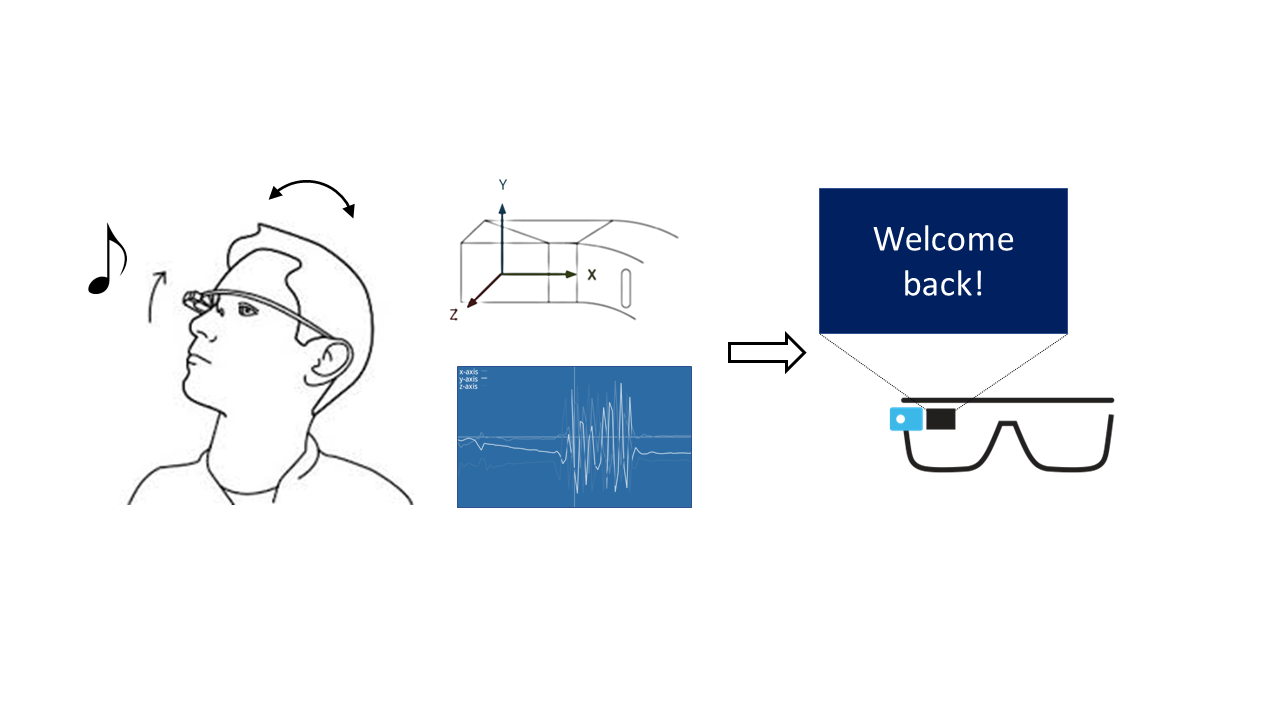
\includegraphics[width=\columnwidth]{figure/headbanger_illustrate.png}
\caption{Illustration of Headbanger. The head-worn device authenticates the
users based on signatures generated from head-movement patterns.  These patterns are created in
response to an audio snapshot played on the device.}
\label{fig:headbanger-illustrate}
\end{figure}

We therefore focus on a third class of direct authentication methods: relying upon the uniqueness of human behavior characteristics such as human walking gait, arm swings, typing patterns, body pulse beats, eye-blinks, etc. This way of authenticating users is often referred to as \emph{behavioral} biometrics, and existing work has largely studied it in the context of authenticating smart phones and tablets~\cite{rahman2014bodybeat,cornelius2014wearable,stevenage1999visual,okumura2006study,monrose2000keystroke,jorgensen2011mouse,bo2013silentsense,de2012touch}. The main advantage of using behavioral biometrics for mobile devices is that the signatures can be readily generated from raw data of built-in sensors such as motion sensors, camera, microphones etc. Considering that cameras and microphones, as well as vision and audio processing algorithms, are quite energy-hungry, we thus focus on those behavioral biometrics that can be easily captured by sensors that require less power consumption, such as accelerometer. \emph{More specifically, we propose to authenticate wearable devices to users based on one type of behavioral characteristics: our unique body movement patterns and their dependence on external stimuli that wearable devices can generate, such as vibrations and music.}

\vspace{1mm}\noindent{\bf Head-movement based authentication.} Body movement 
patterns have long been used by humans to discriminate between people. By 
watching how a person walks, dances, waves hands, we can often recognize 
the person from afar. This is because human body movements are usually 
\emph{distinctive} and \emph{repeatable}. Achieving the same through 
wearables, however, is not straightforward and poses significant research 
challenges: it is unclear whether these seriously-constrained devices are able 
to capture the movement patterns, process the data, and quantify the 
uniqueness of each user's behaviors. Moreover, each device will have only a 
limited view of body movements, dependent on its mounting position on the 
human body. In this paper, we set out to conduct a holistic study of wearable 
authentication through body movements and to design an accurate, robust and 
light-weight authentication system. A key distinguishing feature of our work 
is that we will also consider stimuli that wearable devices can provide to 
design challenge-response inspired mechanisms, particularly stimuli that are 
difficult to observe even for the closest adversaries. For example, we can use 
fast-tempo music through earbuds to stimulate movements and to make such 
free-style movements more repeatable. 

In particular, we have designed, implemented and evaluated {\em Headbanger}, 
an authentication system that generates a signature from user's 
head-movements. These signatures are used as the behavioral biometric. To 
ensure that the user is proactive in making head-movements we stimulate the 
process by playing a short duration audio track with fast beats. The user in 
response to the rhythm and beats makes head-movements that are captured by the 
accelerometer and processed to
generate and authenticate the user's unique biometric signature. Although we 
use a Google Glass a running example for the wearable device, our design can 
be applied to other head-worn gadgets and any system that can record 
head-movements through motion sensing. Our choice for using head movements is 
motivated by the fact that head-worn wearables are becoming very common today 
and such devices are already equipped with motion sensors; for example, 
personal imaging and heads-up display devices, gaming headsets, artificial 
intelligence devices.

%Unlike physiological biometrics that require custom hardware,
%behavioral biometrics offer a much more available/conveient solution. The
%challenge, however,
%is to ensure that these patterns are repeatable under all circumstances that
%the user encounters as well as the differentiability factor between different
%human beings. %We show that by using the same external stimulus among all
%%users
%the baseline for comparison is achieved much easier and the head-patterns are
%more consistent and differentiable among users.

%Subconscious head-movement, or any body movement as a matter
%of fact, can be very random in general.
% Our design assumes that there is only one owner per glass, and we can easily
%extend our scheme to handle the cases with multiple owners.

In summary, the key contributions of this paper are:

\begin{enumerate}

\item We have designed and implemented a novel user authentication method to wearable devices
using head-movement patterns. Our study shows that user's head-movement patterns
contain unique signatures that when inferred correctly can be used as valid
behavioral biometrics for authentication. We design a system, \systemname,~ 
that records, processes, generates unique signatures, and classifies 
head-movement patterns of users based on the accelerometer (inbuilt on the 
wearable device) sensor readings.

%\item We devise of a set of light-weight preprocessing and classification 
%algorithms that can effectively transform raw and noisy sensor data into 
%accurate authentication results. We aggressively optimize the processing 
%latencies of these algorithms so that they are well suited for wearable 
%devices.

\item %We implement a data collection application on Google Glass that plays a
%fast beat music (preloaded) through the Glass's speakers and simultaneously
%records and filters accelerometer sensor data. We use this data collection app
%in our experiments to evaluate the system. 
Through comprehensive experiments 
involving multiple users and over
different system design parameters we show that head-movement patterns
can be used as a behavioral biometric. 
Our approach effectively identifies a wearable device user, with average false 
acceptance rate of 3.9\% and an average true-positive rate of 95.1\%.
%average false rejection rate of 4.9\%.

\item We implement \systemname~on Google Glass and carefully profile the 
execution time of each software module in the implementation. Our measurements 
indicate an average response time of 4.4 seconds on the Google Glass for the 
most accurate results.

%\item We have conducted detailed validation of using head-movement patterns 
%as a biometric characteristic by collecting and analyzing data from multiple 
%users. We will make these data publicly available, which may facilitate other 
%user behavior studies.
\end{enumerate}

%In the sections to follow, we will discuss the background of wearable
%device authentication in section~\ref{sec:background} and details of our
%proposed system design in section~\ref{sec:design}. We evaluate the system in
%section~\ref{sec:results} and follow up with discussions and conclusions in
%sections~\ref{sec:disc} and~\ref{sec:conc}, respectively.












\iffalse
Wearable devices are typically user-interface constrained
Unlike a smartphone, touch gestures or voice activation or face
recognition units not all wearable devices today have the generic
user interfaces such as touch or audio or visual so that typical
gesture or

The recent years have seen a significant growth in popularity of
smart wearable devices. This growth can be attributed to the advances in
hardware miniaturization technology as well as economically affordable
and energy efficient sensing and computing. While size, energy and cost
constraints remain key motives for improvements in wearable computers'
design, the aspect of user authentication has received relatively less
attention. Wearable devices often collect and store sensitive data about
users, and thus there is an obvious need to authenticate the right user to the
device. Solutions today primarily rely on indirect authentication
mechanisms through the user's smartphone, which can be cumbersome and less
secure. Biometric based solutions, though very effective, however, are subject
to the availability of the specific sensors in the wearable unit. In this
paper, we propose to authenticate wearable devices to users based on their
unique behavioral patterns. In particular, we prototype an authentication
system for wearable devices by monitoring user's unique head-movement patterns
in response to an external audio stimulus. Using a personal imaging device as
a running example, and through extensive experimental evaluation over multiple
users, we show that our mechanism can authenticate users with high accuracy


\fi 
\section{Background}
\label{sec:background}

\subsection{Mobile Device Authentication Through Body Movements}


%\begin{comment}
%\end{comment}

%Authentication mechanisms for wearable devices can broadly be divided into two
%categories: (i) {\em Direct} authentication, where the users can directly
%authenticate themselves to their wearable device using the input/output
%interface and/or using signatures generated from the sensors available on the
%device, and (ii) {\em Indirect} authentication, where a secondary device --
%typically the user's smartphone -- is used as a medium for authentication.
%Today's commercially available wearable devices predominantly use the latter
%approach where users login to their wearable devices through their smartphone
%-- using a PIN or an email account.
%%A select few gadgets, for example the Google Glass or fitbit, require the
%%users to register their device to their user specific accounts (gmail for
%%Google Glass), which can also be perceived as an indirect mechanism for
%%authentication.
%Unlike the indirect approaches, that require users to have multiple devices, direct
%mechanisms only rely on the wearable device by leveraging the inbuilt interfaces and sensors on the
%wearable device.

%%One form of direct authentication is the well-known
%%the PIN code approach, however, its effectiveness is only limited to the PIN
%%being safe-guarded by the user. A slightly more effective approach would be
%%to use a randomly generated code for the user, similar to the RSA
%%%keys~\cite{},but that would require a secure and stable wireless connection
%%%to the server.
%The fact that wearable devices relate significantly to ``what we wear" on the
%human body, biometrics can play a key role for direct authentication to
%wearable
%devices.

%Biometrics allow a system to identify a user based upon ``who you
%are" (i.e., her physiology) instead of ``what you
%have'' (i.e., ID cards) or ``what you know'' (i.e.,
%passwords)~\cite{jain2004introduction,o2003comparing,yampolskiy2007motor}.
%Physiological biometrics such as DNA, ear shape, face, fingerprint,
%hand or finger geometry,
%iris, odor, palm-print, retinal scan, and voice, have been very effective and
%widely used in many prototype and commercial authentication systems.
%In addition, body shape such as body height, width, and body-part proportions
%can also be used as biometric cues to identify different
%people~\cite{collins2002silhouette}. Even characteristics such as
%body weight and fat percentage have been considered as secondary biometrics
%for authentication purposes~\cite{ailisto2006soft}.

%However, biometrics are
%not prominently used in wearable devices that are commercially available
%today, though
%there have been specific point commercial designs (e.g., Nymi~\cite{nymi}). This can be attributed to the
%fact that biometrics would require the specific hardware and sensors available on
%the wearable device. Also the overheads for physiological biometrics in
%wearable devices can be high, in both, cost for hardware as well as
%integration and computing.

%%Most of the afore-mentioned biometrics, however, require extra hardware
%%(e.g., camera) and/or processing that is too demanding for wearable devices.

A number of body-movement based authentication approaches have been proposed for mobile devices. These systems
leverage unique signatures from human behavior that may be subconscious
or in response to external stimulus or both.  For example, it has been shown that gait (e.g.~stride length, the amount of arm swing) when the user is walking or
running is a reliable identification cue, and irrespective of the
environment~\cite{stevenage1999visual}. Okumura et.al.~\cite{okumura2006study}
have shown that human arm swing patterns can be used to create signatures
to authenticate to their cell-phones. Monrose
et.al.~\cite{monrose2000keystroke} show that keystroke rhythms, when
users type on the keyboard, that include typing dynamics such as how
long is a keystroke, how far is between consecutive strokes, and how is the
pressure exerted on each key, can be used to authenticate
users. Similarly, mouse usage dynamics~\cite{jorgensen2011mouse} and touchpad
touching dynamics~\cite{bo2013silentsense,de2012touch} have also been shown to
serve as potential authentication cues.

We take the viewpoint that, in comparison to other means of authentication, body-movement based
authentication may offer great convenience. With increasing access to built-in sensors on wearables, it
has become possible to generate and infer unique behavioral signatures
specific to users. With this rationale, we design an authentication system, dubbed {\em Headbanger}, for head-worn
devices by monitoring user's unique head-movement patterns in response to an
external audio stimulus.

%\vspace{4pt}{\bf Head-movements as a behavioral biometric.}
\subsection{Using Head-movement for Authentication}
\label{subsec:headmovements}

%As such, authenticating a user involves comparing her sensor
%readings with the pre-recorded glass owner's sensor readings.
%Our design assumes that there is only one owner per glass, and we can easily
%extend our scheme to handle the cases with multiple owners.
%Figure~\ref{fig:sysarch} presents the system architecture of the \systemname,
%and in the following section, we will discuss each component of this design
%in more detail.

According to Jain et al.~\cite{jain2004introduction}, a type of body movement is useful for
authentication when it is \emph{universal}, \emph{distinctive},
\emph{repeatable}, and \emph{collectible}. %With the advancements in head-worn
%wearable computer designs, collecting head-movement
%patterns using built-in accelerometers and motion sensors has become increasingly
%accessible. 
Sensors for collecting head-movement patterns are
available on most of today's head-worn wearable devices, and thus
making head movements both {\em universal} and \emph{collectible}.

In this paper, we show that free-style head movements are  \emph{distinctive} and \emph{repeatable}, especially when combined with external stimuli such as music beats. In~\systemname, music plays a crucial role in stimulating body movements such that the resulting movement pattern is natural to the user (more distinctive) and easier to remember (more repeatable). Zentner and Eerola~\cite{zentner2010rhythmic} have shown that most people move
their body as a natural response to external rhythmic stimuli such as music;
even at a very early age, infants respond to music and their movements speed
up with the increasing rhythm speed. Most adults naturally perform head
movements or hand movements when listening to a fast beat audio track \textbf{FIXME, citation needed here}.  When
combined with external rhythmic stimuli, we believe body movements become more
distinctive -- not only a person's movement pattern is unique, but their
response to rhythmic stimuli is also unique. In this way, the resulting
authentication system will be more dependable.

\begin{figure*}[t]
\begin{center}
\begin{tabular}{ccc}
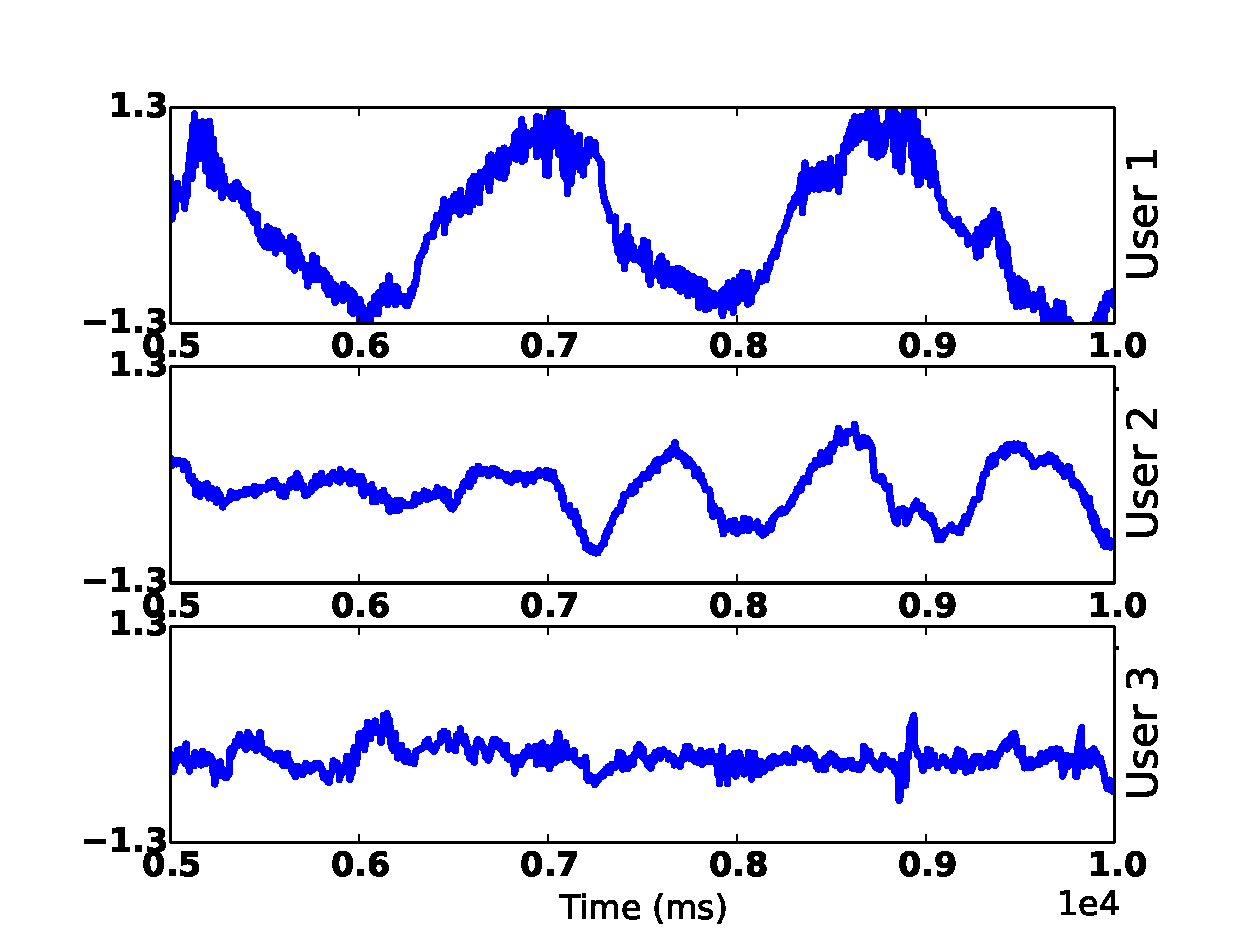
\includegraphics [width=.33\linewidth]{figure/raw_x.eps}&
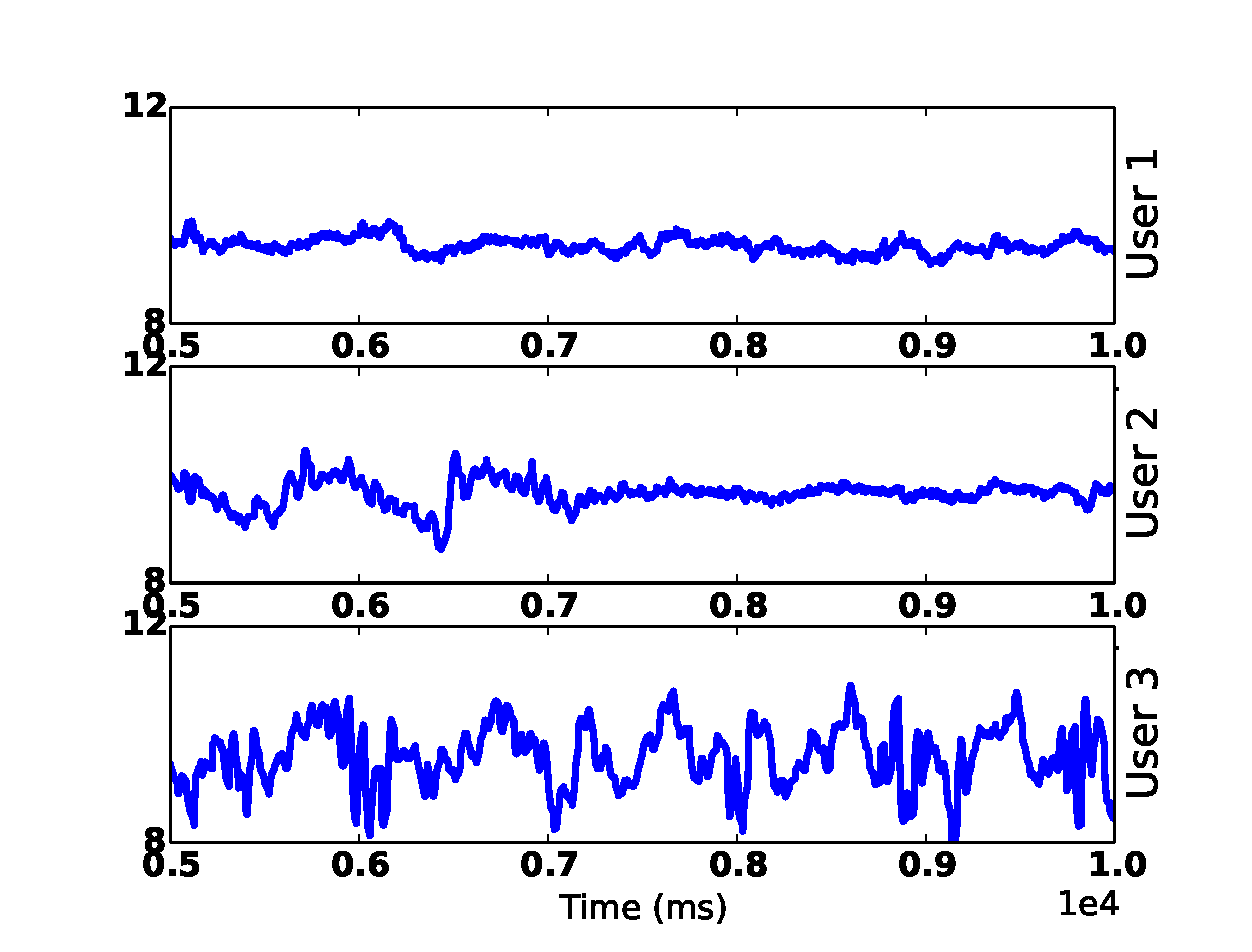
\includegraphics [width=.33\linewidth]{figure/raw_y.eps}&
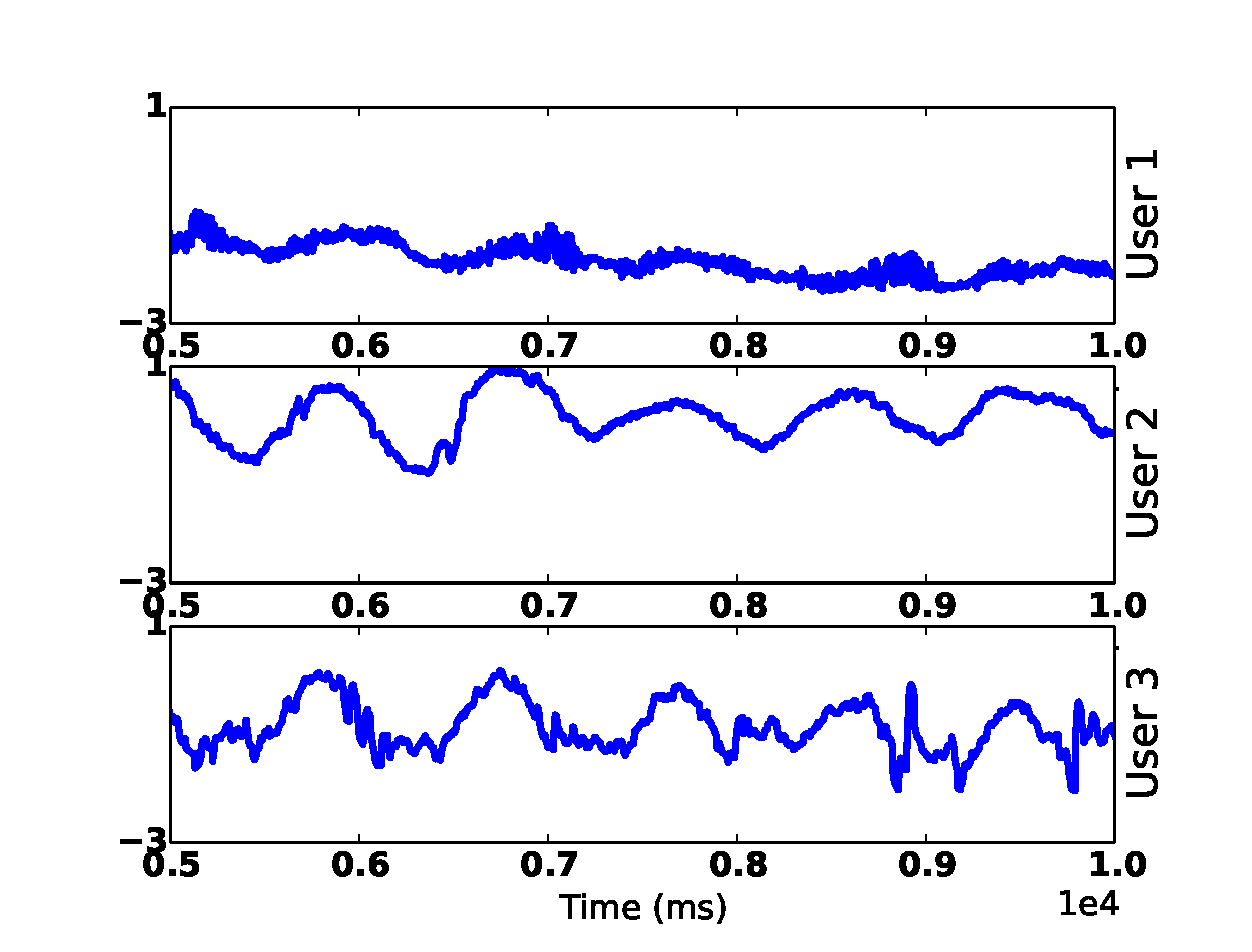
\includegraphics [width=.33\linewidth]{figure/raw_z.eps}\\
(a) X-Axis & (b) Y-Axis & (c) Z-Axis \\
\end{tabular}
%\begin{tabular}{cc}
%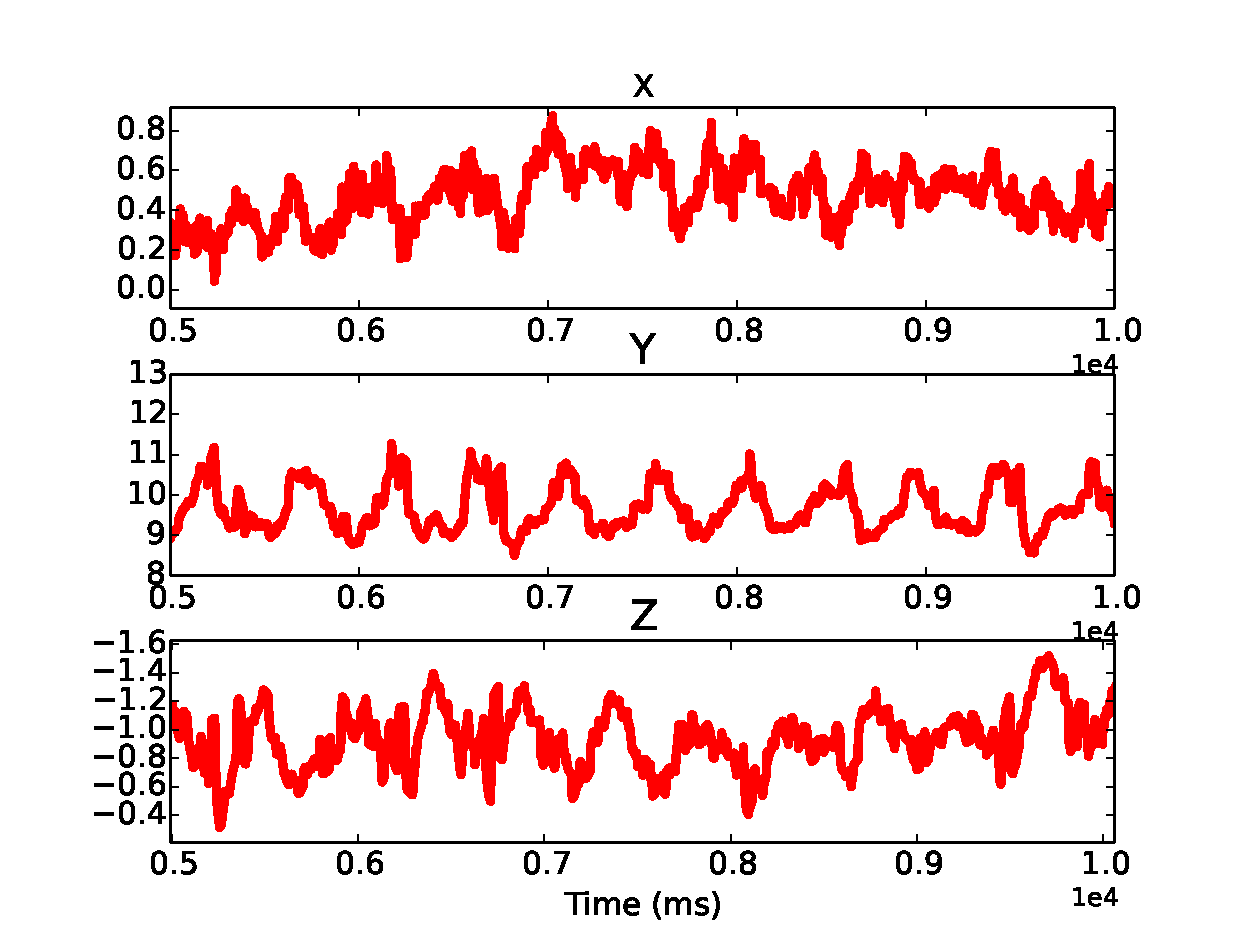
\includegraphics [width=.33\linewidth]{../fig/raw_sub4.eps}&
%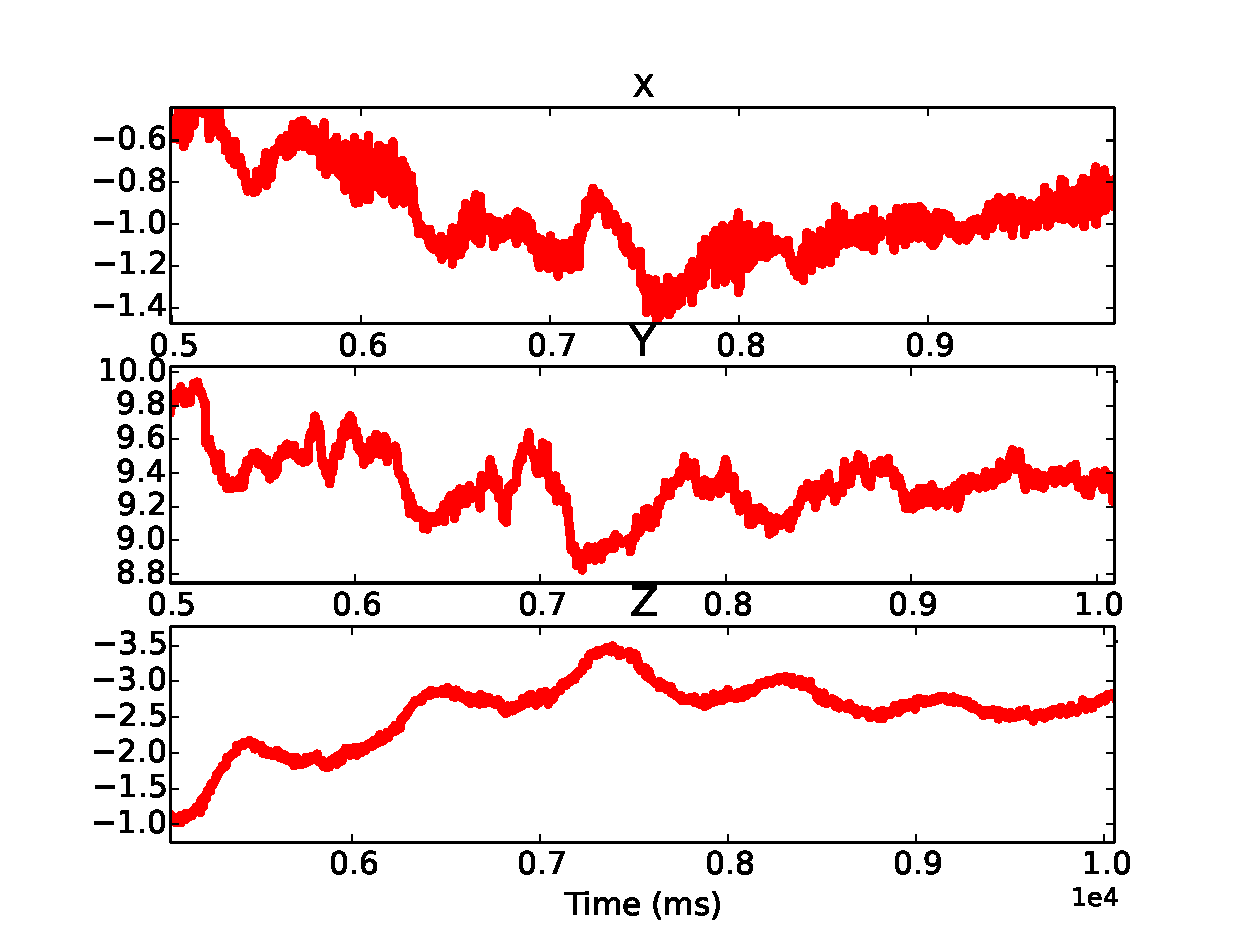
\includegraphics [width=.33\linewidth]{../fig/raw_sub5.eps}\\
%(d) User 4& (e) User 5 \\
%\end{tabular}
\end{center}
\caption{\label{fig:raw} These plots show the raw accelerometer data in the
time domain for five different users when they move their head in response to
the same music track wearing the same Google glass. The plots
indicate that different users' head movement patterns appear distinctive from
each other. The three users wore a Google Glass (in turns) and listened to a
10 second audio snapshot of a pop song.}
\vspace{-2pt}
\end{figure*} 


Based on a preliminary analysis of the accelerometer signals from three Google Glass
users, we observed (see Figure~\ref{fig:raw} (a)-(c))
that these users {\em repeatedly} showed {\em distinctive} head-movement patterns
(that are differentiable even through simple signal processing techniques),
when listening to the same music beats.

%Motivated by this observation we hypothesize that head movements
%can be a good behavioral biometric characteristic to authenticate
%users to their smart glass.
%We next formally present the design of our system that
%utilizes head-movement patterns as behavioral biometric signature
%to authenticate smart glass users.




%\section{Preliminary Study}
%In order to understand the insightful information of musical head movement,
Next, we conducted a preliminary experiment to further investigate whether head-movement patterns can be potentially used to authenticate users. In this experiment, we collected head-movement accelerometer data from 28 subjects, wherein each subject was asked to perform a simple nodding movement following a short audio track (referred to as \emph{music cue} in the rest of the paper).   For this purpose, we examined %two simple features: (1) wave amplitude, the difference between the bottom of a wave and the peak of the following wave, which indicates how hard a person nods; %(2) mean wave width, the mean interval between two consecutive wave bottoms or peaks, which indicates the length of a nodding motion;
%and (2)
a simple aspect of the head-movement pattern, response time, which is the time interval between a music beat and the corresponding nodding motion, as shown in Figure~\ref{fig:waveform}. The response time indicates how quickly a person responds to music beats.
% we extract several characteristics from the original accelerometer data:
%\begin{itemize}
%\item{\em Wave amplitude},which is the difference of a wave bottom and its next wave peak. It measures the acceleration when the user performs the head-movement, in other words, wave amplitude describes “how hard” the user nod his head. Due to accelerometer data usually contains high frequency noise, and we are more interested in the main signal where user nod his head, a 5-Hz-cutoff low-pass filter is applied before we extract all the characteristic in the signal.
%\item{\em Wave widh}, which is the time interval between two bottoms or two peaks. It describes the time to complete one nodding movement. The user is stimulated by a music cue, wave width is effected by the time interval between beats.
%\item{\em Series of response time (SRT)},which is the series of time interval between the music beat and corresponding movement.  Studies in ~\cite{westeyn2004recognizing} and ~\cite{wobbrock2009tapsongs} show SRT could be used to differentiate the users. It is important to note that user is not necessary perform after the music beat. The evidence in music psychology ~\cite{clarke1999rhythm,fraisse1982rhythm} demonstrate that  humans have capability to perceive and perform rhythmm, hence user can perform the moving before he hears the beat.
%response time in our measurement can be either negative or positive. However, finding the associated movement of a beat is a non-trivial process, hence we develop the following algorithm to achieve this goal and form a SRT. First, accelerometer data needs to be synchronized with the music cue in midi format. Since midi file is a time series of instrument commands,  no additional signal processing is required to detect the beat in the music as we can take each command as a beat if the music is simple enough. Second, we locate two neighboring peaks where a beat resides in between, and compute the time intervals from the beat to both peaks. Finally, we choose the one with a smaller absolute value as the response time. Note that we only use data from two axis, since nodding rarely generates meaningful data on the other one. In some cases,  user is not necessary nodding for every beat,  thus we use the 90 percentile of the response time sample to interpolate  when the detected response time is beyond this value.
%\end{itemize}
<<<<<<< HEAD
\begin{figure}
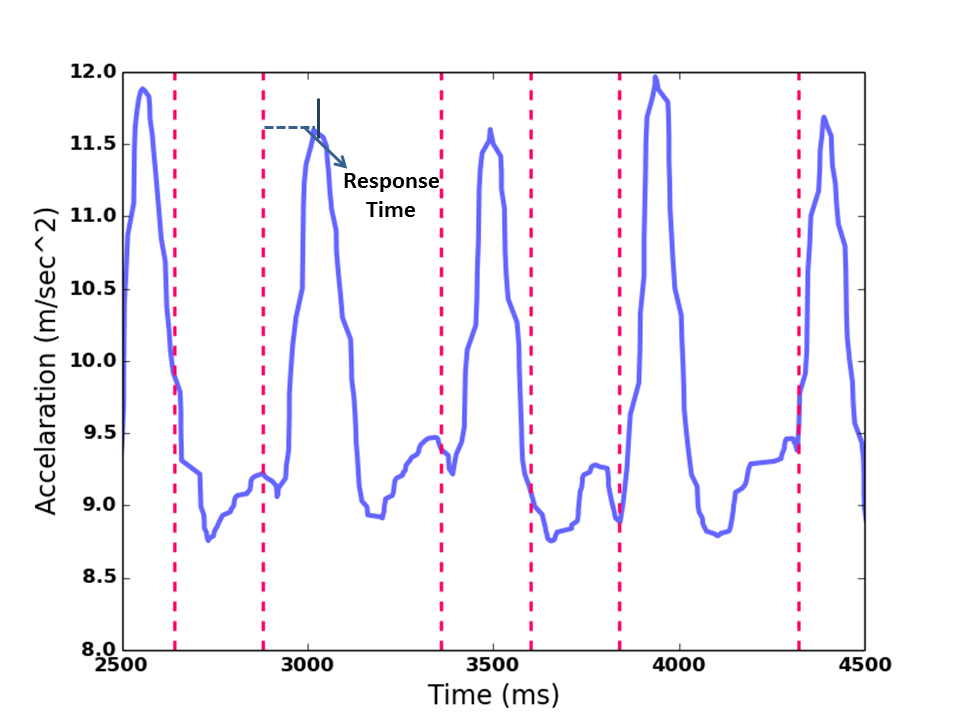
\includegraphics[width=.75\columnwidth]{figure/waveform_1.png}
\centering
\caption{\label{fig:waveform}Waveform with beats snapshot. Response time is determined by the time interval between a beat and its closest wave peak. }
=======
\begin{figure}[t]
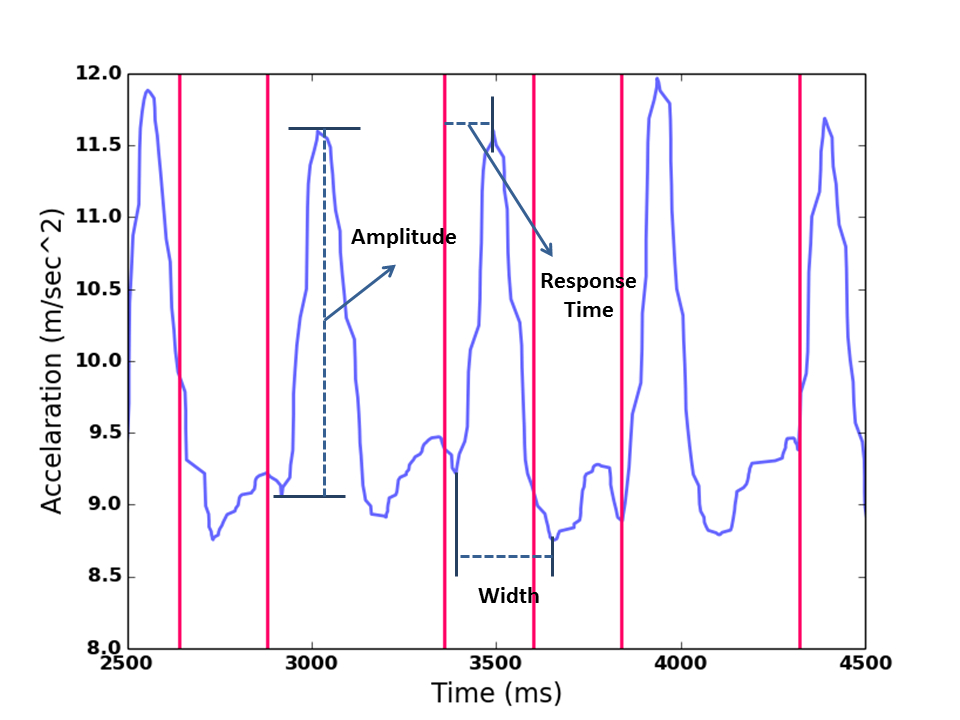
\includegraphics[width=.75\columnwidth]{figure/waveform_resp.png}
\centering
\caption{\label{fig:waveform}Response time of a head motion is the interval between the motion and the music beat to which the motion responds. From a sequence of head motions, we can obtain the response time time series.}
>>>>>>> 68513003dc6ad372dcd15fe264feeb2235311e94
\end{figure}

%\begin{figure}
%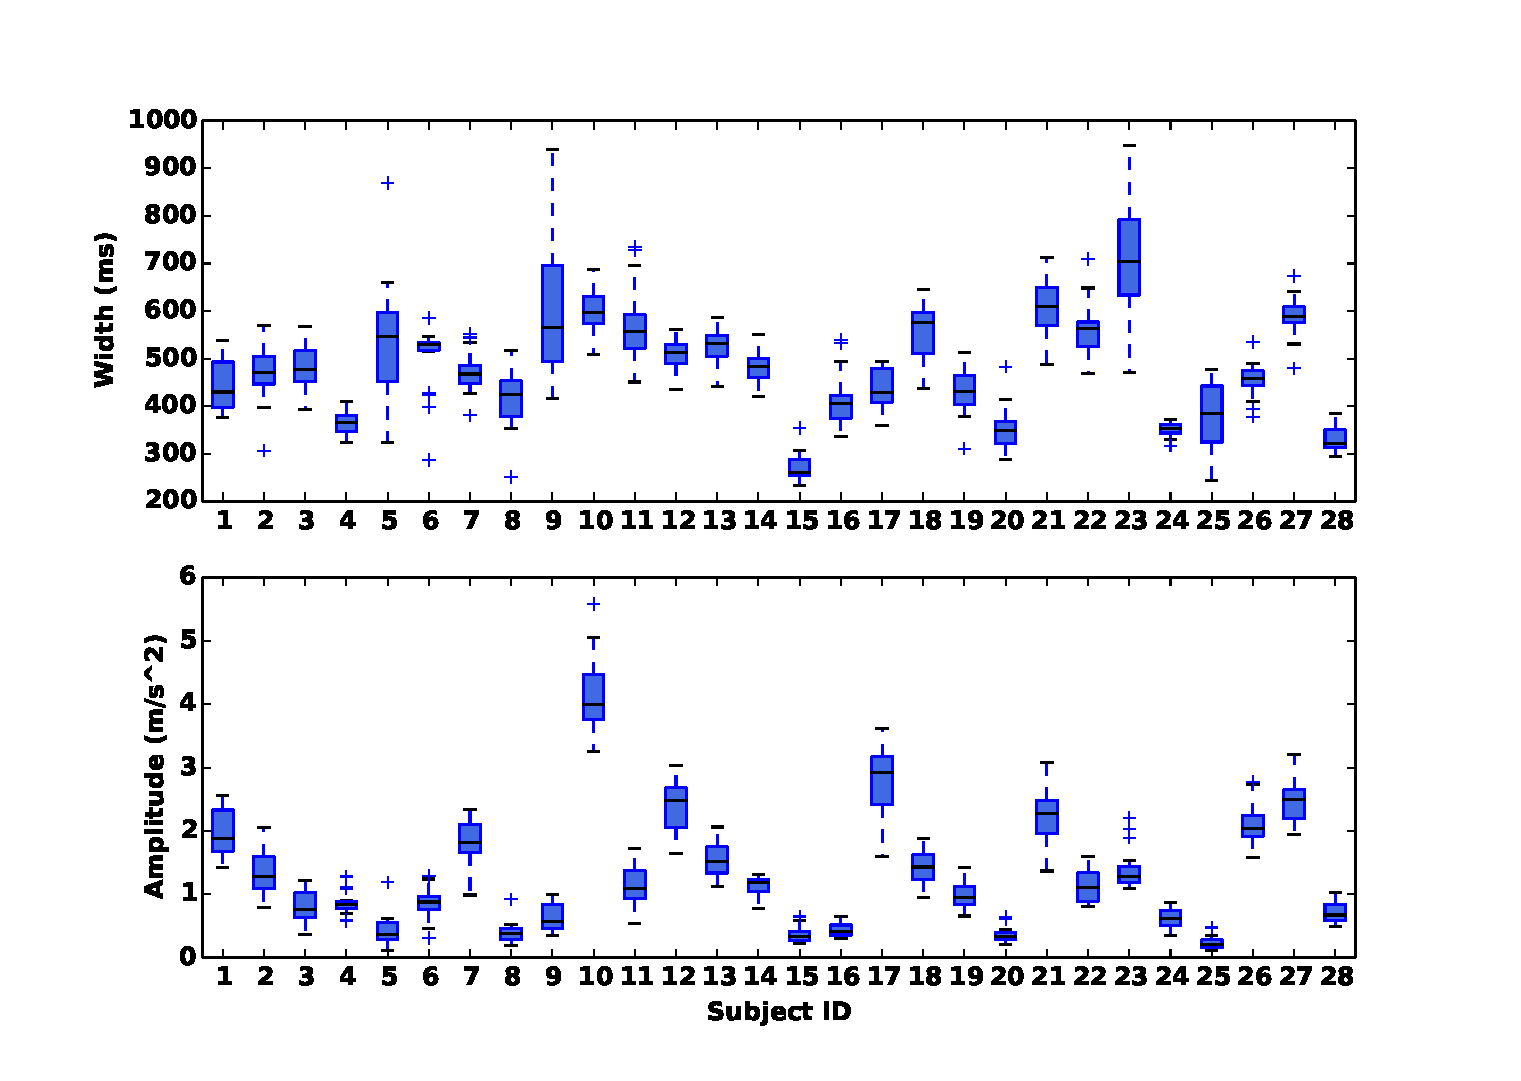
\includegraphics[width=\columnwidth]{figure/width_amp_box.eps}
%\centering
%\caption{\label{fig:width_amp} Wave Amplitude Boxplot **YZ: please re-consider the features** \textbf{ALL FIGURES SHOULD TELL WHAT IS THE TAKE-AWAY. MAKE THE PAPER GLANCEABLE, INCLUDE A PARAGRAPH FOR ALL FIGURES}}
%\end{figure}

\begin{figure*}[t]
\begin{center}
\begin{tabular}{ccc}
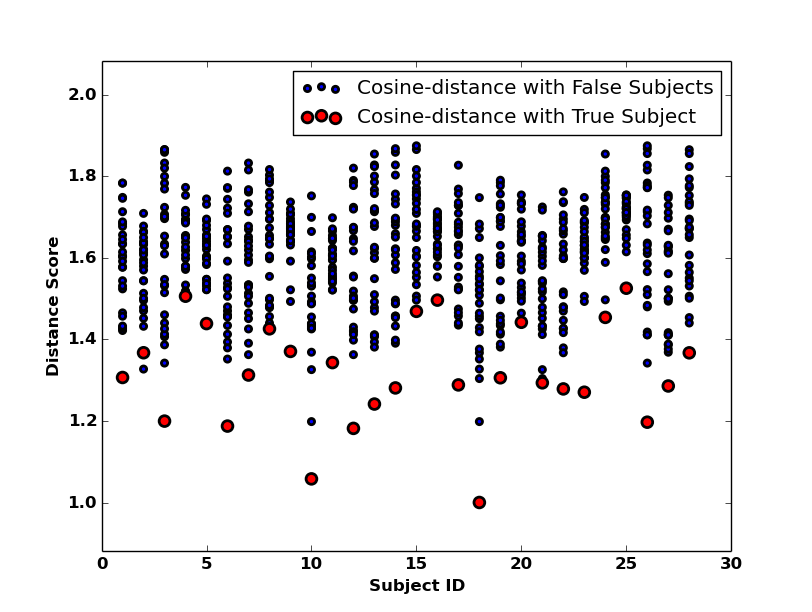
\includegraphics [width=.31\linewidth]{figure/resp_time_cos.png}&
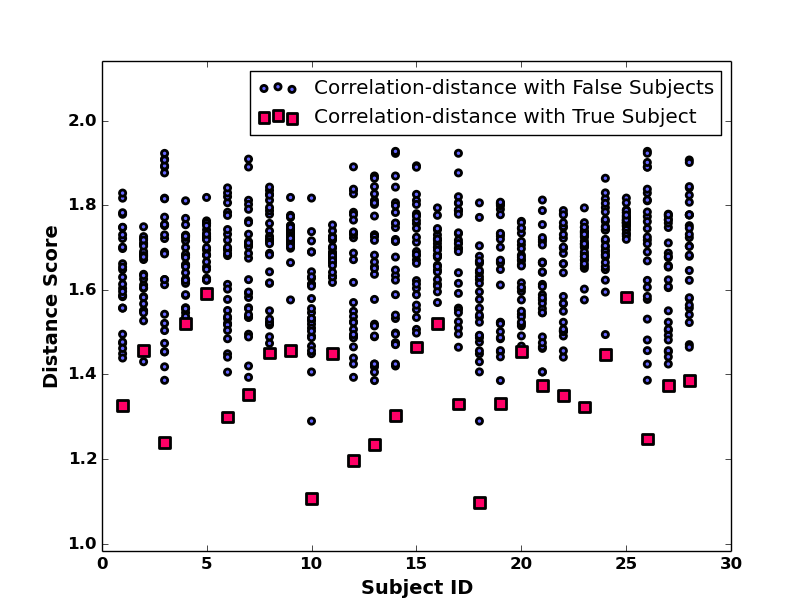
\includegraphics [width=.31\linewidth]{figure/resp_time_cor.png}&
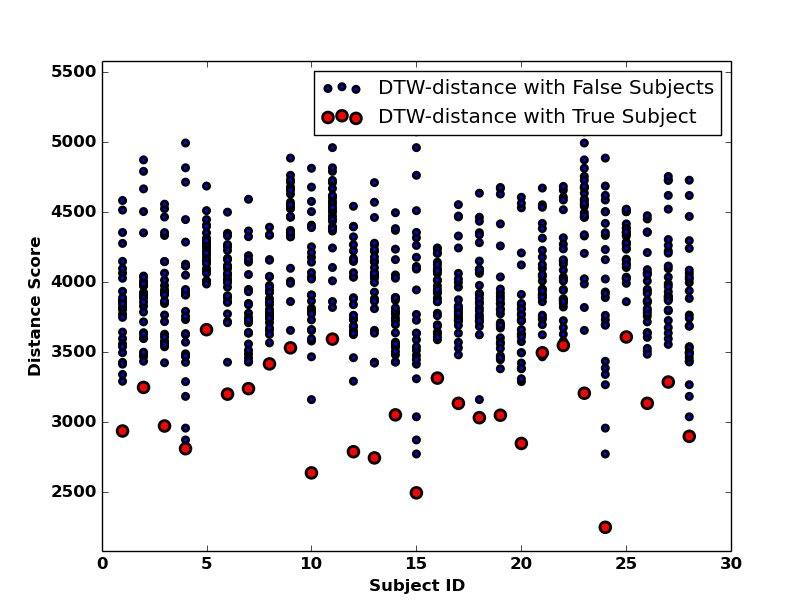
\includegraphics [width=.31\linewidth]{figure/resp_time_dtw.png}\\
(a) Cosine Distance & (b) Correlation & (c) DTW \\
\end{tabular}
\end{center}
\caption{\label{fig:distance} (a) Cosine, (b) Correlation and (c) DTW distances are computed over 20 response time time series for each subject, with 28 subjects in total. For each subject's column, a red dot represents the average distance among that subject's own response times, while a blue dot represents the average distance to other subjects' response times. The results show that red distances are always lower than blue ones, suggesting that different subjects' head-movement patterns are distinguishable.}
\vspace{-2pt}
\end{figure*}


%Figure~\ref{fig:width_amp} shows each subject's wave amplitude box plot (we collected 20 nodding samples for each subject in the experiment). We observe that each subject's wave amplitude distribution ***

Next, we calculate the distances between response time time series of different subjects. Specifically, we take the response time time series of each subject, and calculate the average cosine distance (COS), correlation (COR), and dynamic time warping (DTW) output~\cite{dtw} between any pair of subjects. **** We plot these three types of distance values in Figures~\ref{fig:distance} (a)-(c). In each plot, we show distance values for all 28 subjects -- for each subject, we plot the average distance between her response time time series and time series from each of the other 27 subjects (referred to as distances with false subjects, shown in blue dots), as well as distances among her own response time time series (referred to as distances with true subjects, shown in red dots). All three figures show that distances within a subject's own response times are clearly smaller than those across subjects.

These observations suggest that even with simple nodding movements, the accelerometer data collected by Google Glass have the potential to be used as authentication means. With this motivation, we next devise the authentication protocol for \systemname.
%To better understand the SRT for different users,  we apply various similarity scores to provide an intuitive and quantitative description of their difference. In Figure~\ref{fig:distance}, the average Cosine Distance (COS) and Correlation (COR) can help most of the subject to differentiate himself with the other subjects, but for some subjects's true subject score (red dot) are closed to their false subject score (blue dot). For subject 2, red dot even exceeds the blue dot.The output of Dynamic Time Warping (DTW)~\cite{cite dtw} can be used as another distance metric.In Figure~\ref{fig:resp_time_dtw},  it shows that all average self-comparing similarity scores are lower than that when they are compared with false users. In real world, the SRT detection algorithm may not be practical if we also consider more complex head-movement other than simple nodding for each beat. The observation above indicates the possibility to further derive a system which can differentiate the true user and the false users based on the fusion of these characteristics. 
\section{Headbanger System Design}
\label{sec:design}

\begin{figure}[t]
\centering
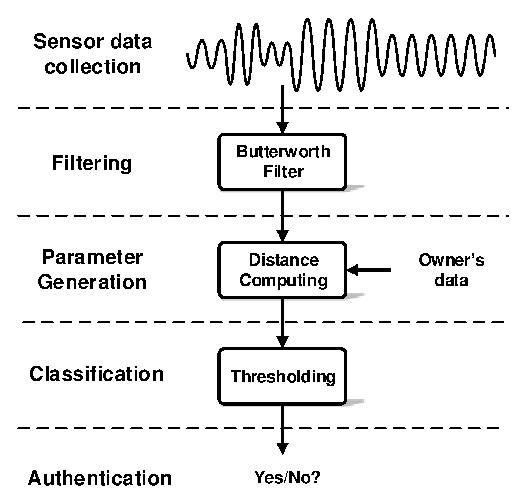
\includegraphics[width=0.75\columnwidth]{figure/system.eps}
\caption{\systemname~system design flow. The online authentication phase of \systemname~consists of the following steps: (1) sensor data collection in which we collect accelerometer data while users move their head as a response to an audio track played on the glass, (2) filtering in which we apply a Butterworth filtering to smoothen the sensor data for subsequent processing, (3) parameter generation in which we calculate the distances between two accelerometer samples as the parameter, and (4) classification in which we adopt an adaptive thresholding mechanism to classify the user's head movement, whose output will be used as the authentication result.}
\label{fig:sysarch}
\end{figure}

%\begin{figure*}[t]
%\begin{center}
%\begin{tabular}{ccc}
%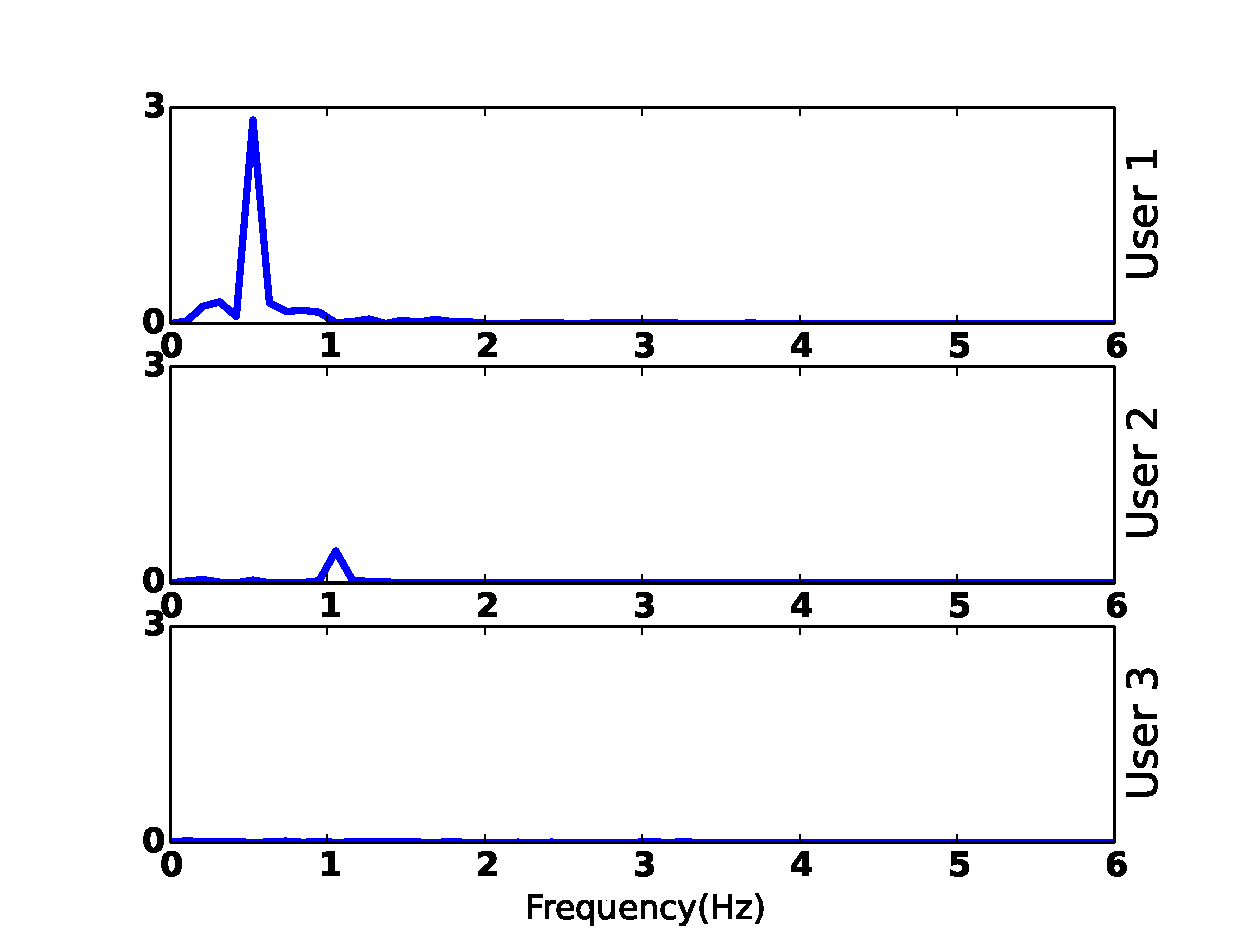
\includegraphics [width=.33\linewidth]{figure/freq_x.eps}&
%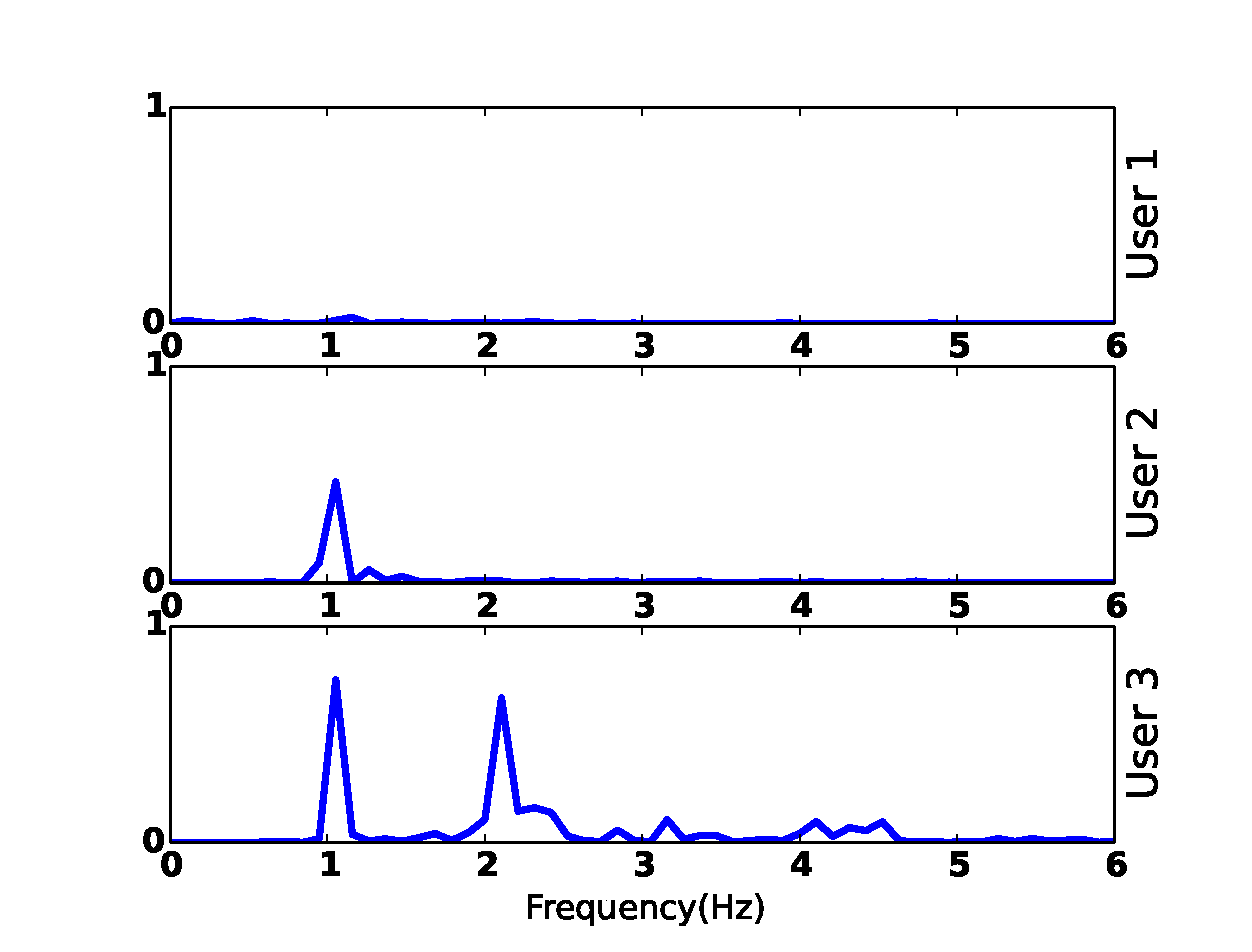
\includegraphics [width=.33\linewidth]{figure/freq_y.eps}&
%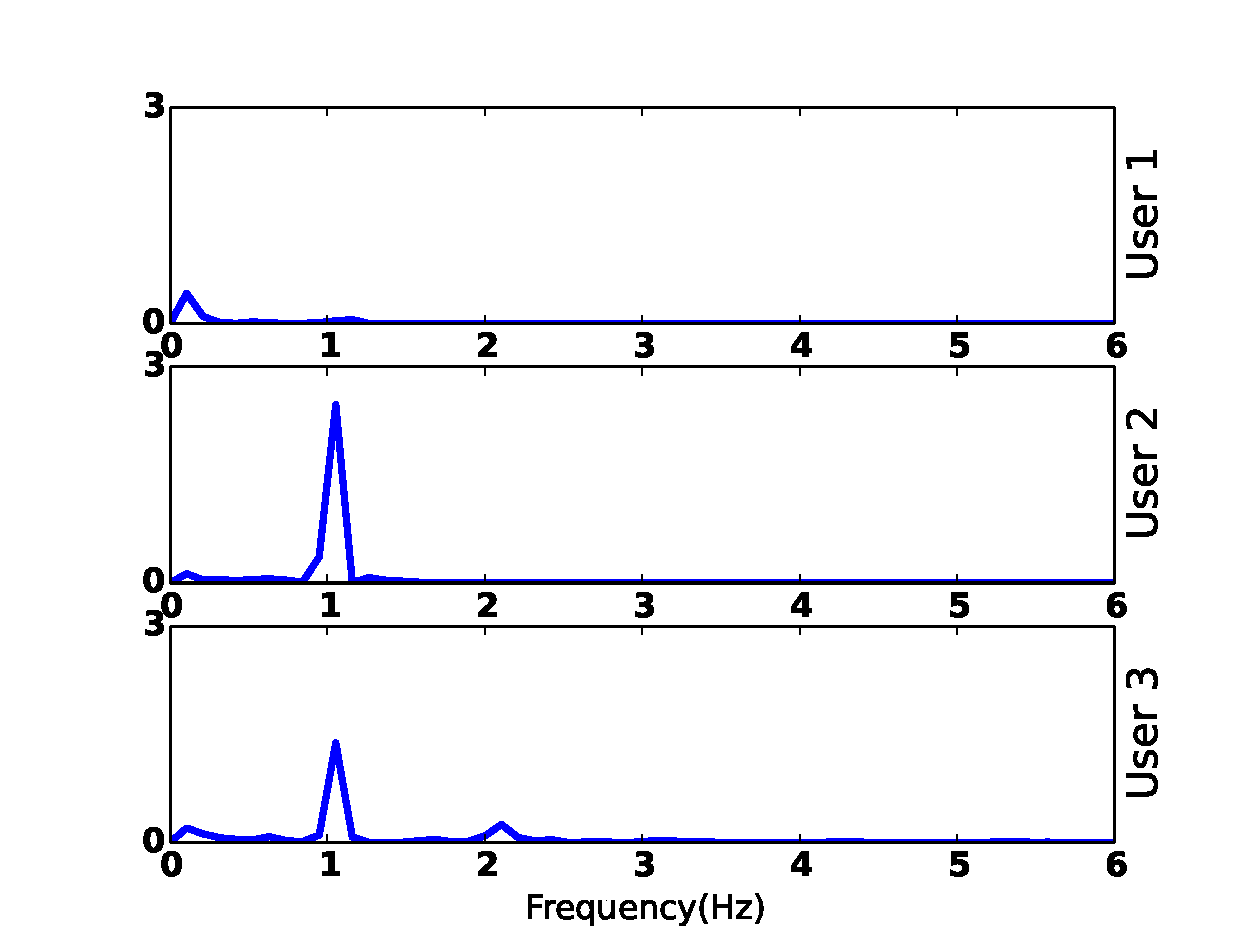
\includegraphics [width=.33\linewidth]{figure/freq_z.eps}\\
%(a) X-Axis & (b) Y-Axis & (c) Z-Axis \\
%\end{tabular}
%\end{center}
%\caption{\label{fig:raw_freq} Accelerometer data from three users, in the frequency
%domain. The data show that the spectrum is significantly
%concentrated within 5Hz for all three users.}
%\end{figure*}

\systemname~enables direct authentication of users to their smart-glass devices or smart-glass apps using
head-movements. We posit that \systemname~will run as a service in the device upon power-up or application start-up,
similar to the screen-lock in smartphones.  %The authentication process is initiated
%by playing a short music cue, to which the user
%responds through head-movements.


 %We envision that our proposed system will be used as an authentication
%interface on the smart-glass wearable device.
The authentication process has two phases: an offline training phase and an
online authentication phase. In the training phase, the system
collects sensor readings when the real user moves her head with a music cue (following her pre-designed movement pattern), and uses the collected data to
build a classifier. In the following discussion, we assume there is only
one real user for the device for the sake of simplicity. An extension to
support multiple users per device can be realized through minor modifications,
namely, by appropriately indexing the users in the trained database.

In the online authentication phase, we collect sensor samples during a user's authentication attempt and label the samples using the \systemname~classifier.
The user is authenticated upon a successful classification.
 %Our design is developed based on the idea that humans respond to music
%naturally through head movements, and that such movements are more
%significant and unique when the track contains fast beats and/or rhythm.
%We will refer to the audio snapshots as {\em music cues} in the rest of the
%paper.
%~\systemname~generates unique features from the head
%movements of a user, and uses them as a unique signature for
%identifying the right user of the device. The system will
%grant access only when the head-movement signature
%generated during the login attempt matches with the
%original user's signature.

As illustrated in Figure~\ref{fig:sysarch}, \systemname~involves the following key modules: sensor data collection and filtering, sample distance computing, and classification.
%\begin{itemize}
%
%\vspace{-2pt}\item {\em Sensor data collection}: ~\systemname~records the head-movements
%in the form of raw accelerometer signals (in 3 dimensions) using the inbuilt
%accelerometer
%sensor on the smart-glass device.
%\vspace{-2pt}\item {\em Filtering}: The accelerometer signals are filtered by applying
%a low-pass filter to remove records of extraneous motion.
%\vspace{-2pt}\item {\em Parameter generation}: The accelerometer signals are
%processed through the dynamic-time warping (DTW) tool~\cite{dtw} to obtain a
%DTW feature that is treated as the unique signature for the user.
%%A user can generate different signatures for different audio tracks. A
%%training phase collects the set of signature for each user-audio pair.
%\vspace{-2pt}\item {\em Classification}: The signatures are classified as
%a match or not a match, based on a thresholding
%scheme and using the trained data set as a reference. The system grants the
%user access to the device if there is a match
%with sufficient confidence.
%%In the former case, the system will grant the user access
%%\item {\em Authentication}: The head-movement signature generated
%%during system operation is compared with the original user-audio pair
%%signature, and the user is authenticated access if there is a plausible match.
%\end{itemize}
%
%The original signature of the glass user is generated through a
%training phase that is executed when the glass is operated
%by the user for the very first time, and the training data gets
%updated upon each use of the device.
%As shown in Figure~\ref{fig:sysarch} shows the block diagram of
%~\systemname system design.
We will now discuss these design aspects in more detail.
\subsection{Sensor Data Collection and Filtering}
%To facilitate natural head movement, we provide several
%short music tracks with easy-to-follow beats.

The data collection step involves collecting motion sensor data (we mainly focus on accelerometer in this study) while the user makes head-movements
in response to the music cue  with a duration of $T$ seconds.
The raw accelerometer
signals are collected at
a sampling rate of $r$ samples/sec. %; the default sampling rate on Google Glass is 50Hz. 
The accelerometer data corresponding to one user,  is a
collection of accelerometer readings on the
3D axis (x, y, and z) collected over $T$-second duration, 
%Figure~\ref{fig:headbanger-illustrate} illustrates the axis
%conventions with respect to the user's head position.
%The data collection unit stores
stored in a matrix with dimensionality $3\times rT$. %where each element corresponds
%to one signal point.
We will refer to this $3\times rT$ matrix as a {\em sample}.
We retain the duration $T$ to be in the order of few seconds, as frequency of
human head movements are, intuitively, typically in the order of few times per
second. %This intuition will be more clear from the filtering stage to be
%discussed next.
%The sensor data is accumulated in a $30r$ matrix, which we refer to as
%one $ACC$ sample.
%We hypothesize that
%head-movement can serve as a reliable behavioral biometric -- that is, $ACC$
%samples from the same user have smaller distances than samples from different
%users.

%\begin{figure*}
%\begin{center}
%\begin{tabular}{ccc}
%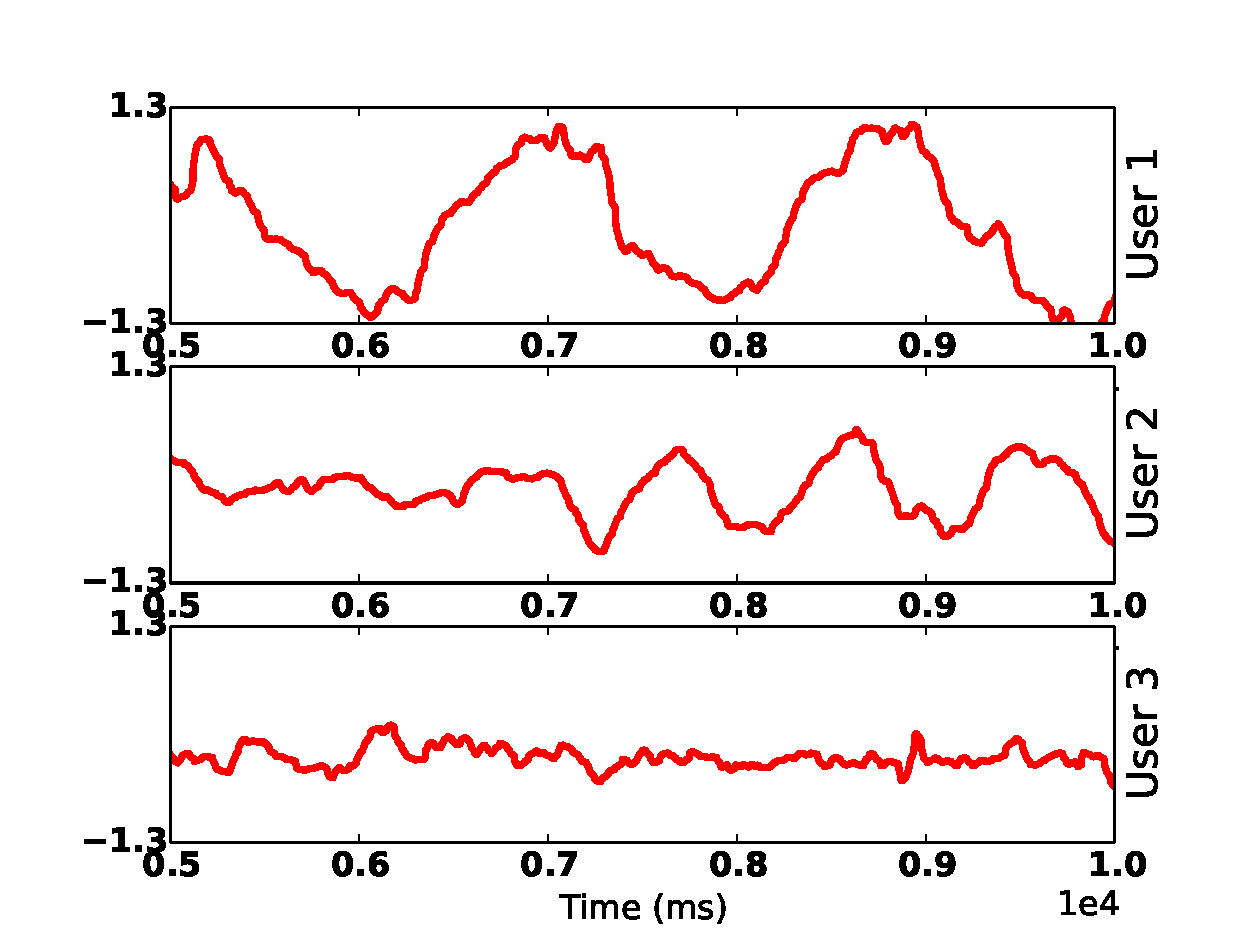
\includegraphics [width=.33\linewidth]{figure/filtered_x.eps}&
%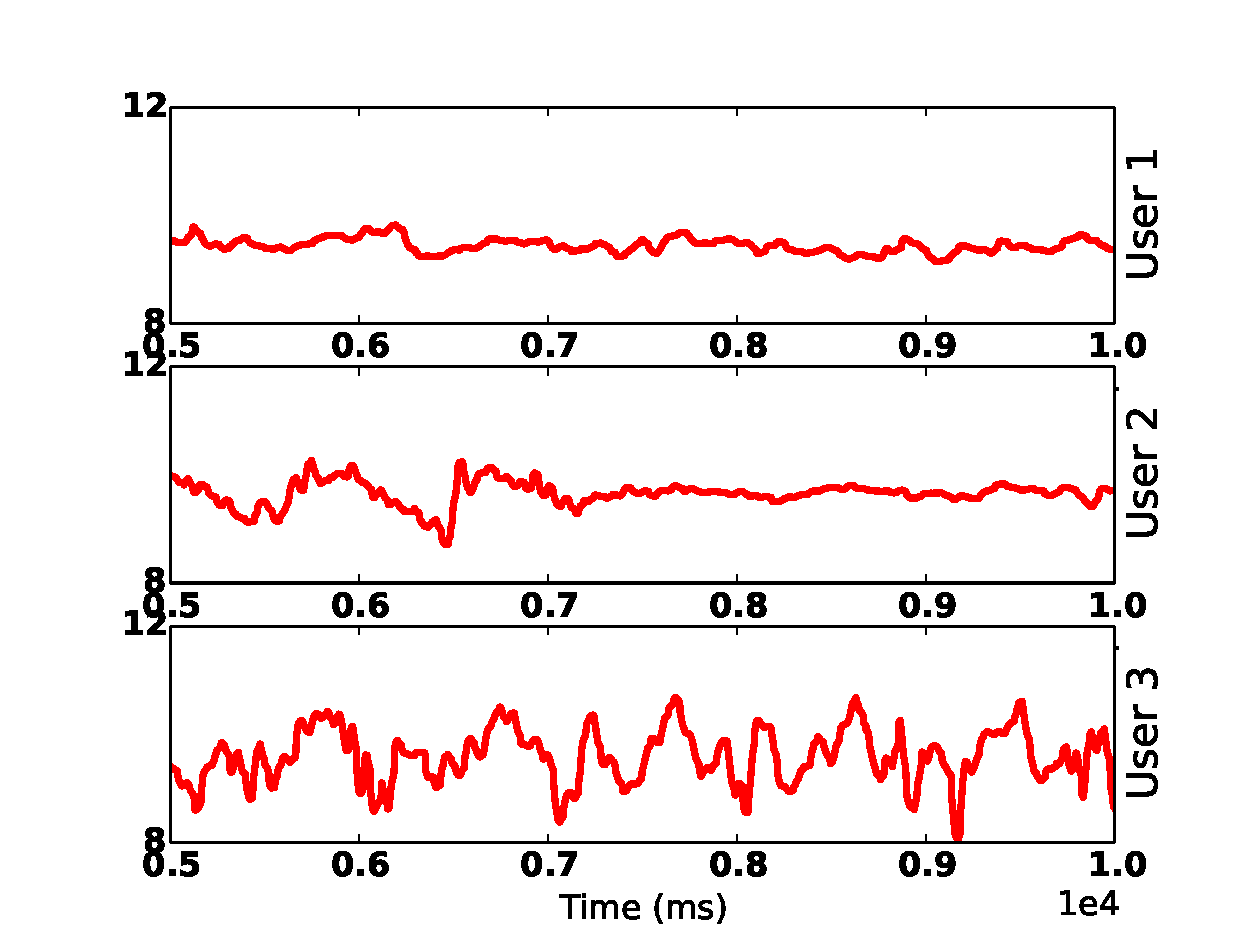
\includegraphics [width=.33\linewidth]{figure/filtered_y.eps}&
%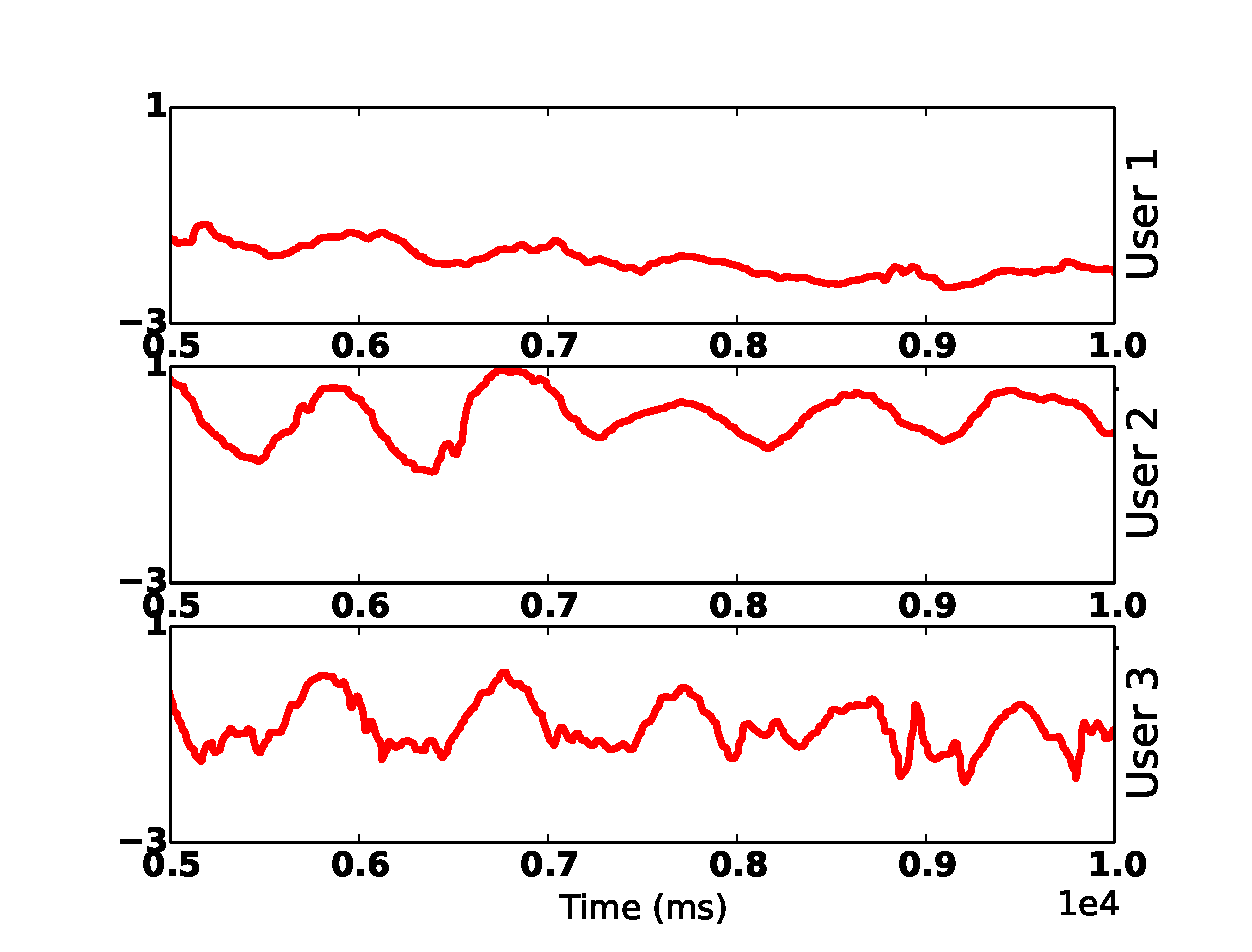
\includegraphics [width=.33\linewidth]{figure/filtered_z.eps}\\
%(a) X-Axis & (b) Y-Axis & (c) Z-Axis \\
%\end{tabular}

%\iffalse
%\begin{tabular}{cc}
%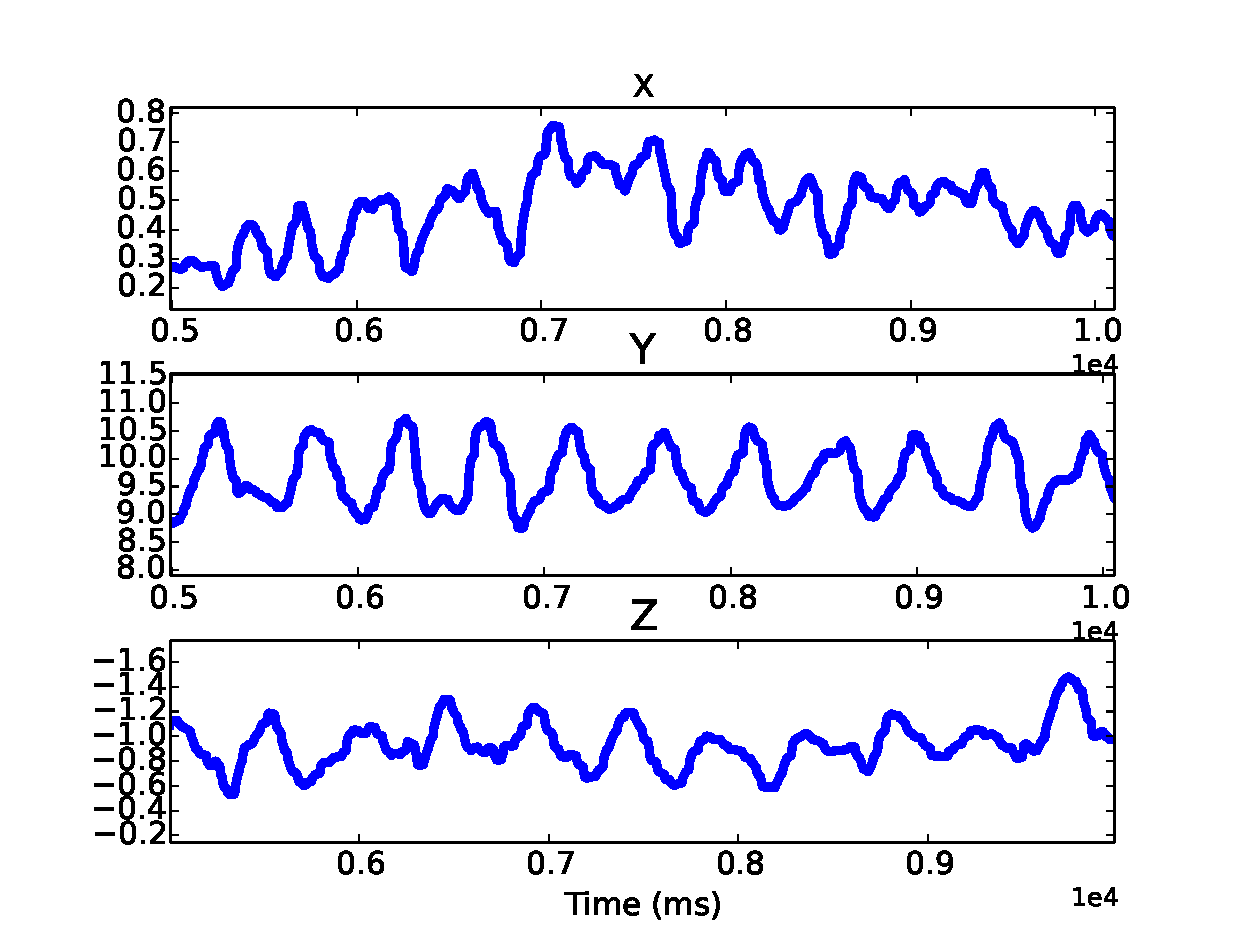
\includegraphics [width=.33\linewidth]{../fig/filer_sub4.eps}&
%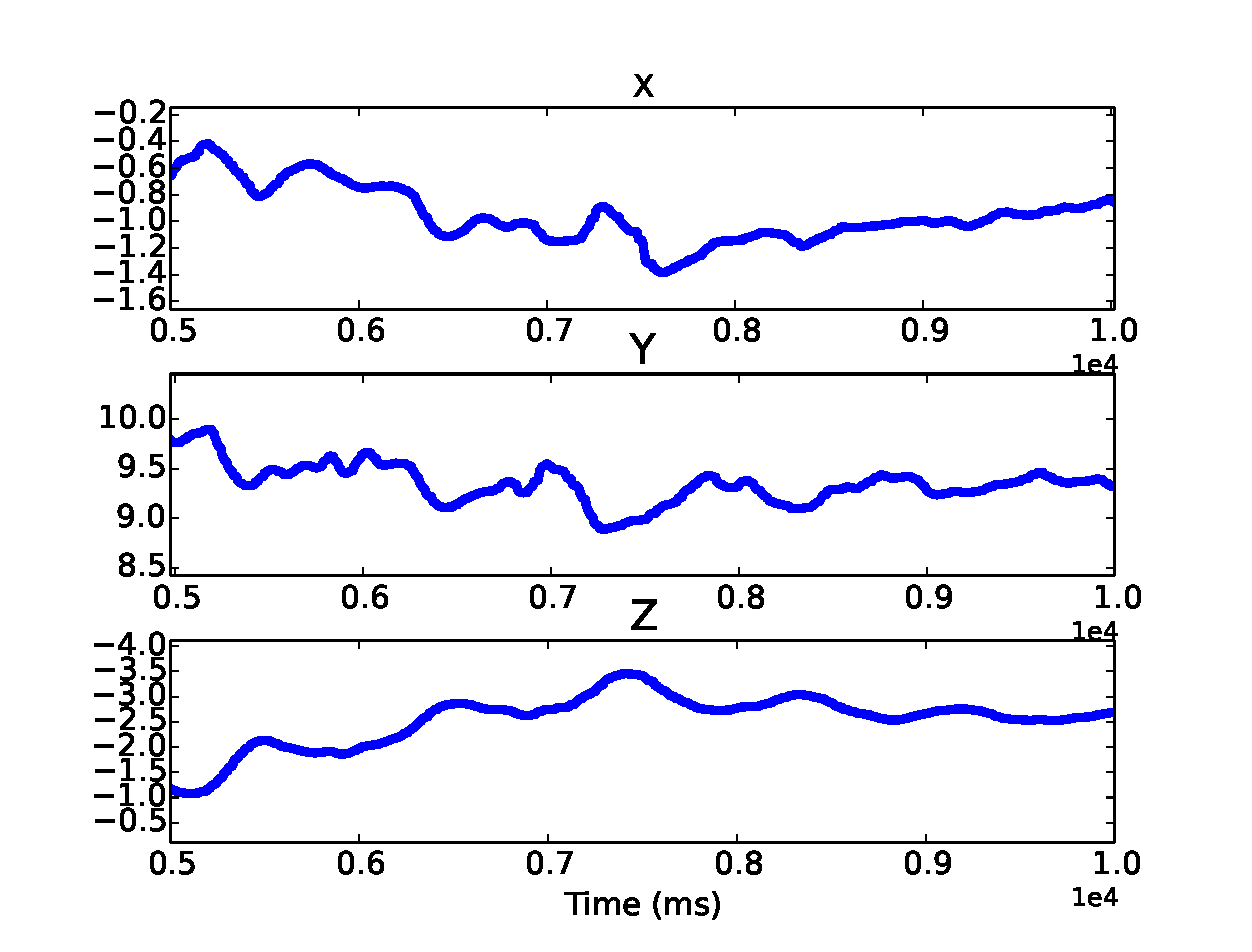
\includegraphics [width=.33\linewidth]{../fig/filer_sub5.eps}\\
%(d) User 4& (e) User 5 \\
%\end{tabular}
%\fi
%\end{center}
%\caption{Filtered accelerometer signals. Applied Butterworth
%filter of order 2 and cut-off frequency 10Hz.
%\label{fig:filteredacc}}
%\end{figure*}


%\subsection{Filtering}

Next, we filter the raw samples to remove noises due to spurious movements such as vibration or shaking.
%The filtering ensures that the head-movement signature
%generated from the accelerometer readings encompasses
%only head movements, and not any spurious signals caused due to
%vibration or shaking.
%From the frequency
%spectrum of each accelerometer sample, as shown in
%Figure~\ref{fig:raw_freq}
%for three users, we can observe that the spectrum is significantly
%concentrated within 5Hz.
%We note that music tracks with high tempo, or fast beats, typically contain
%beats in the order of the order of hundred beats per minute.
%In particular, the high tempo music that we used in our experimentation was
%contained 94 beats per minute~\cite{beats}.
%We infer that the head-movement, in response
%to the beats, will be of the same order. Hence, we hypothesize that
%the signal spectrum in [0,5] Hz range encompass
%human head movements; where 0 Hz can indicate that the head is
%steady still, and 5 Hz can correspond to a vigorous head-shake.
We adopt a low-pass digital Butterworth
filter~\cite{challis1983design} and set a relaxed cut-off frequency of 10Hz.
%Even with the relaxed cut-off, the filtering results in
%clean accelerometer samples with head-movement patterns
%that are prominent and detectable.
%Figures~\ref{fig:filteredacc} (a)-(c) show the filtered results of the raw accelerometer
%samples shown in
%Figure~\ref{fig:raw};
%compared to raw data, the filtered results are much more
%suitable for subsequent processing.

%\begin{figure}[t]
%\centering
%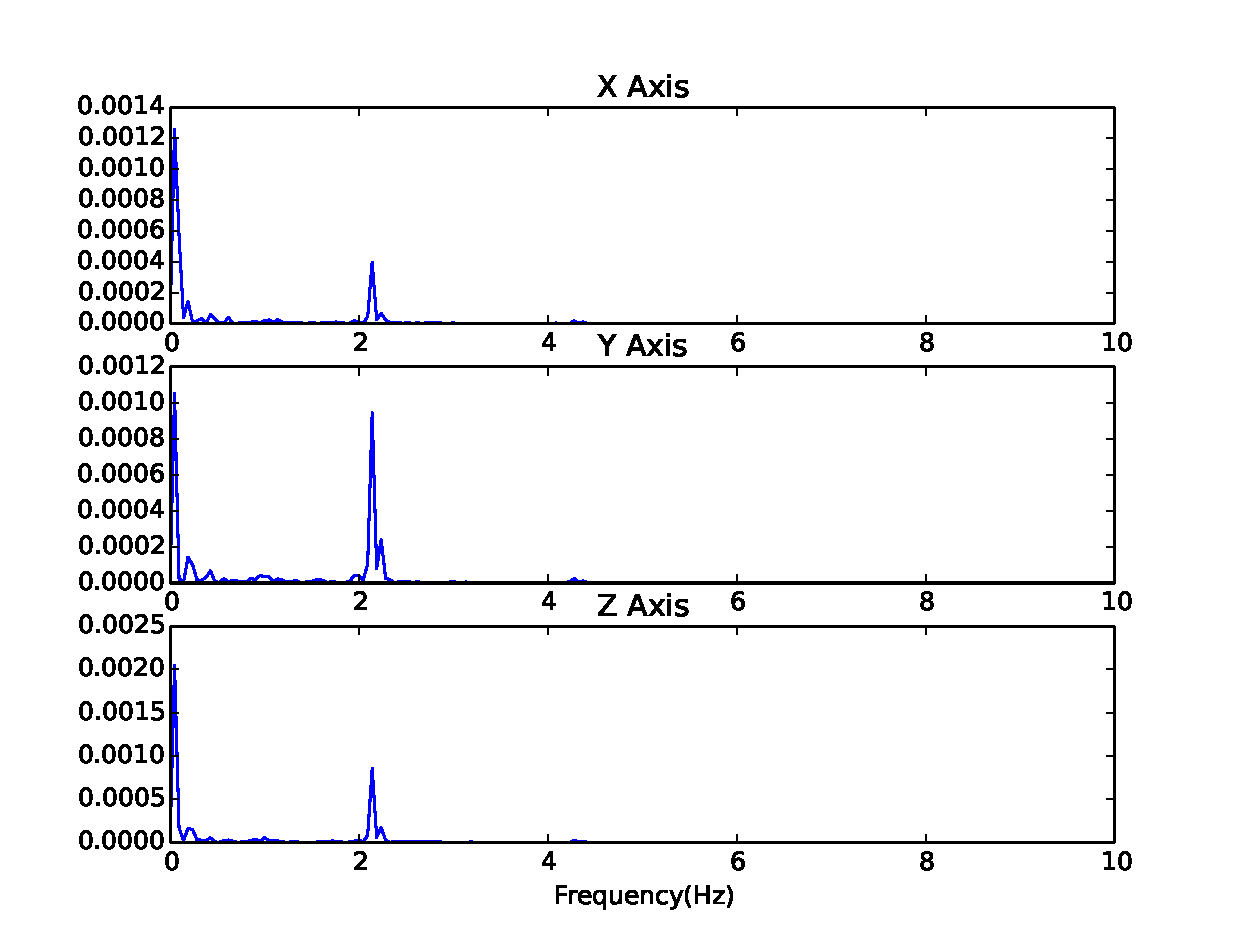
\includegraphics [width=.95\linewidth]{fig/freq_resp.eps}
%\caption{\label{fig:freq_resp}Fiver users' $ACC$ samples in frequency domain.}
%\end{figure}

\subsection{Sample Distance Computing}\label{subsec:distance}
%\subsection{Quantifying Sample Similarity}


In this study, we build a distance-based classifier for its simplicity is well suite for wearable devices. There are various ways of computing distances between two signals; we have considered three popular distance-computing algorithms in this study -- Cosine (COS)distance, Correlation (COR)distance, and dynamic-time warping (DTW)distance.

Suppose we have two time series $S_a = (s_1,s_2, ... ,s_n)$ and $S_b = (s_1, s_2, ..., s_n)$.  Their COS distance is calculated as $\frac{S_{a}\cdot S_{b}}{\left \| S_{a}\right \|\times \left \| S_{b} \right \|}$;   The COR distance is calculated by dividing their distance covariance by the product of their distance standard deviations; The DTW distance is defined as the distance when the optimal alignment between $S_a$ and $S_b$ has been determined by "warping" them non-linearly.   ~\cite{dtw}.
%We generate a signature from the accelerometer signals using the
%dynamic-time warping (DTW) tool~\cite{dtw}. DTW is generally used
%as a similarity matching tool for time-domain analysis of
%temporally varying signals.
%DTW compares a temporal signal with a reference (temporal) signal over a
%certain time-window and yields a distance measure as the score. A low score
%(DTW distance) implies that the test signal is in close match with the
%reference.
%We use the DTW to generate a signature for the head-movements
%from the accelerometer signal.
%We observed from our preliminary tests that, users often
%start head movement at an angle with the vertical which varies among users.
%However, we also observed that the head-movements that follow exhibit a
%consistent, and often periodic, patterns over time.
%We empirically observed that the accelerometer signal patterns
%are consistent after the first 1sec duration of head-movements.
%Treating the accelerometer sample set from the first trial as a reference, we
%apply the DTW algorithm on the successive accelerometer sample set to obtain a
%distance score vector, $\hat{d} = (d_x, d_y, d_z)$; the three elements in
%$\hat{d}$ denote the DTW distance score in the $x, y, z$ axes, respectively.
%By computing the mean of the distance scores obtained for each accelerometer
%pair we generate the mean-value DTW distance, which is treated as the
%head-movement signature or unique {\em feature} for that particular user and
%audio
%combination.

%In the offline training phase, we conduct
%%For evaluation purposes, we conduct an elaborate training phase where
%$M$ trials of head-movement exercises, collect $M$ training samples, and
%obtain $M-1$ reference distance vectors. We observed from our evaluations (to
%be discussed in the next section) that $M = 30$ can yield in high accuracy
%while $M = 10$ can yield reasonable accuracy. The trade off is the computation
%overhead that goes into conducting the training (primarily DTW computations)
%for the $M$ samples.
%In real usage of the application,
%the user would conduct only
%two trials of $T$ duration each where trial 1 is treated as reference.
%In this way, the training can be done in-situ. The training data-set is
%updated upon each usage of the authentication interface.
%%Small distance values DTW is expected to return relatively small distance
%%values for samples from the same user, while returning large distance values
%%for samples from different users (that have different movement patterns).
%%Here, $S1$ is the reference

\iffalse
Next we investigate how we can accurately quantify the similarity level
between two accelerometer samples, whose results will be used to classify the users.
After testing various methods,
We decide to adopt the Dynamic Time Warping (DTW) algorithm that is
often used to measure similarity between two waves based on temporal
stimulation.  Unlike many other algorithms, DTW measures the similarity
between two signals that are similar but with phase difference, which is well
suited for our study. In our study, users often start head movement at a
different angle, but exhibit similar, often periodic, pattern for a similar
amount of time. Applying the DTW algorithm on two accelerometer samples $S1, S2$, we
get a vector $(d_x, d_y, d_z)$ denoting the distance in the $x, y, z$ axes
respectively. DTW is expected to return relatively small distance values for
samples from the same user, while returning large distance values for samples
from different users (that have different movement patterns).

YZ: Sugang, we need some detailed equations or algorithms here.
\fi

\subsection{Classification}
The classification step labels a test sample as ``true'' or ``false'' depending upon whether its distance to the real user's training samples is below a threshold. Again, we choose this method because it strikes a good balance between simplicity and performance. Next, we explain how we build the classifier and how to conduct online classification in detail:
%In this study, we developed a simple yet effective classification scheme based on adaptive thresholds.

\begin{enumerate}

\vspace{3pt}\item \emph{Identifying Top-$K$ Training Samples.} Given $M$ training samples, we first identify the $K$
samples that are closest to all the training samples. For each training sample, we calculate its average distance to the other $M-1$ samples, and then choose those $K$ samples that have the lowest average distance values. These $K$ samples are empirical estimation of the centroid of the sample space, and thus best represent the space among the collection of the training samples. We refer to them as Top-$K$ samples. In our classifier, we focus on the Top-K training samples instead of all the training samples because it does not only incur much less computing overhead, but it also provides much better robustness against noises in training data.

\vspace{3pt}\item \emph{Establishing Distance Threshold.} Suppose a sample, $s$, is one of the Top-K samples. We have its distance scores to the other $M-1$ samples in the training set, from which we can calculate the distance mean $\mu_s$ and distance standard deviation $\sigma_s$. Then sample $s$'s distance threshold is defined as ($\mu_s+n\sigma_s$), where $n$ is referred to as the threshold parameter for our distance-based classifier.

\vspace{3pt}\item \emph{Classifying Test Sample.}   If we use a training sample $s$ to classify the test sample $t$, then $t$ is labeled as a true sample if the distance between $s$ and $t$ is less then $s$'s distance threshold ($\mu_s+n\sigma_s$); otherwise, it is labelled as a false sample. The strictness of this classifier is characterized by
the value of the threshold parameter, $n$; a large $n$ can increase the false
acceptance rate while a small $n$ value can result in a
high rejection rate of true samples. %In our system we aim to reach an optimal
%value of $n$ that can result in acceptable accuracy.
%\item Steps (1) to (3) are repeated when a new sample set is added to the
%training database resulting in an updated threshold. This way, the thresholding
%based classification is adaptive to the user trials. As we will show in our
%evaluations, the thresholding approach is more robust than the SVM approach,
%through both yield reasonable authentication accuracy.

\vspace{3pt}\item \emph{Voting}. We label the test sample according to all $K$ Top-K samples, and the final classification result is the majority decision among all $K$ individual classification results.


%that have
%the lowest $K$ average distance values to the rest of the
%training set. We next calculate their DTW vectors to the rest of the samples in
%the training set to obtain $(M-1)K$ distance vectors. We call this resultant
%vector as Top-$K$ reference distance vector. For example, if $K = 1$, then we
%call the resulting algorithm as Top-1 algorithm; if $K \neq 1$, then we call
%the resulting algorithm as Top-$K$ voting algorithm.
%The voting refers to the procedure that the DTW computation results for each
%sample in the training set is referenced, sorted (in increasing order of DTW
%scores) and the classification (a binary index, match or no-match) is
%performed on the top $K$ entries. The final classification result corresponds
%to the majority vote from the list of $K$ results.
%By using top $K$ samples, instead of all $M$ samples in the training set, we
%significantly reduce the computation overhead in the authentication
%process. In our evaluation, we will study the impact of $K$ value; in
%particular, we evaluate for $K = 1$ and $K = 3$.

\end{enumerate}
Among the four steps outlined above, the first two steps belong to the offline training phase, while the last two steps belong to the online authentication phase.
Finally, if the user's test sample is classified as ``true'' then the user is authenticated to the device; otherwise, the user is rejected.


\iffalse
\subsection{Authentication}

The authentication step results in a binary output that corresponds to
either allowing or disallowing the user to unlock the device.
In this paper, we make two reasonable assumptions pertaining to authentication
on the smart-glass device: (i) homogeneity of
accelerometer sensors for all smart-glasses (from a particular vendor), and (ii)
that the device is registered to the user with an associated PIN or passcode,
and that the head-movement signature is used for secondary verification.
Upon entry of the correct password, the device verifies the identity
of the user based on the head-movement signature.

In the head-movement authentication phase, given a test sample, we classify the sample as true (1) or false
(0) based on one of the two classifiers discussed above. If the result is true, the user is accepted; otherwise
the user is rejected.
\fi

%The authentication mechanism for each of the two classification strategies are
%as follows:

%{\bf SVM.} Given a test sample, classify the sample as true (1) or false
%(0) based on the SVM classifier. %If the result is true, compute the euclidean
%distance between the each of the top $K$ true signatures and the classified
%test signature. If the euclidean distance is below a pre-set threshold
%(obtained empirically from training phase)


%{\bf Adaptive thresholding.} Given a testing sample, calculate the
%DTW distance between the testing sample and the top $K$ representative
%samples. If the resulting distance mean falls within threshold range, then the
%result is ALLOW USER; otherwise, the user is rejected. 
\section{Evaluation}\label{sec:results}

%In this section, we will present our evaluation results of the \systemname. 
We evaluated \systemname~with comprehensive laboratory studies involving 
human subjects. We collected from volunteer participants accelerometer sensor 
readings with Google Glass.
We analyzed these traces offline on a PC.
Our evaluations are primarily aimed at determining the accuracy of detecting 
and differentiating users based on their head-movements, and understand 
the effect of design parameters such as length of the music cue and training 
data-set size, on accuracy. We also measured the response time of our Google 
Glass implementation of \systemname.
Our studies were approved by the Institutional Review Board (IRB) of our 
institution.
%based on profiling the execution time of each key 
%functions associated with \systemname, on the Google Glass device.


\subsection{Method}
%\subsection{Dataset}


\paragraph{Participants}
** LS: need to update these data **
We had total of 30 volunteer participants. The participants list included a total of 19 males and 11 females. 
The average age of the participants was 29.7 years with a standard deviation 
of 9.81 years. The youngest participant was 23 years old while the eldest was 
at 54 years.

\paragraph{Procedure}
Our first experiment setup aimed at emulating the typical usage scenario 
of \systemname~for authentication, where a user conducts head-movements in 
response to a music cue played on the Google Glass device during a login 
attempt. 
%One of the participants executing the experiment trial wearing the 
%Google Glass. %Figure~\ref{fig:setup} shows our experiment setup.
In this experiment, all participants were asked to wear a Google Glass 
device. Participants who originally wore spectacles were asked to remove their
spectacles before conducting the experiment.
The trials were conducted in an academic environment and overseen by one of 
our team members.
The Google Glass ran our data-collection app that played a piece of 
music (music cue) for a specific duration, and recorded the accelerometer 
sensor readings. We conducted these trials for three duration values: 5 s, 
6 s and 10 s. As we will show further, the accuracy of the system can 
significantly improve with the duration of the music cue; longer the duration 
better is the accuracy. 
The sensor readings were recorded into a text file that was stored 
in the Glass's memory and later transported to a PC for offline processing
through a Python script. The experiment was conducted in a well-lit indoor 
academic laboratory environment. 
 
During the course of the experiment, the participants were allowed to take a 
break or withdraw from experimentation if they felt uncomfortable at any 
point; for example, feeling 
dizzy after head-movement for a period of time, not being able to see clearly 
if near-sighted, etcetera. The conductor also allowed the user to take a break 
of about one minute after each experiment trial.
Each trial lasted for the duration of the music cue played on the Glass, and 
a total of 40 such trials were conducted for each of the 30 subjects. 
The experiment lasted over a duration of 60 days, of which 15 
subjects conducted their trials in a single sitting over a period of two 
hours, while the rest of the trails were spread over 3 days on an average per 
subject.
%while, half of the trials of the rest 10 subjects were spread over 2 days.
The experiment yielded three sets of data traces that each correspond to 
the three music cue durations we selected. 

Our second experiment aimed at an practical imitation attack field test scenario. In this experiment, there were three subjects being taken video while they were performing their login movement. The participants were divided into three group, and each group was asked to imitated one of the three users above. During the test, the participants can watch the video for as many time as they want at anytime between two trials. A feedback from our system will be provided after each trail so that the participants can decide whether they need to adjust their movement or not. After total number of trials reached 30 for each participant, the experiment will stop no regardless the participant succeed or not. The investigator was not only recording the total number of successes, but also the number of trail before the first successful login. This experiment is conducted in quite space on campus. We will now discuss our evaluation results for both experiments in detail. 

\iffalse
\begin{figure*}[t]
\centering
\mbox{
\subfigure[Top 1]{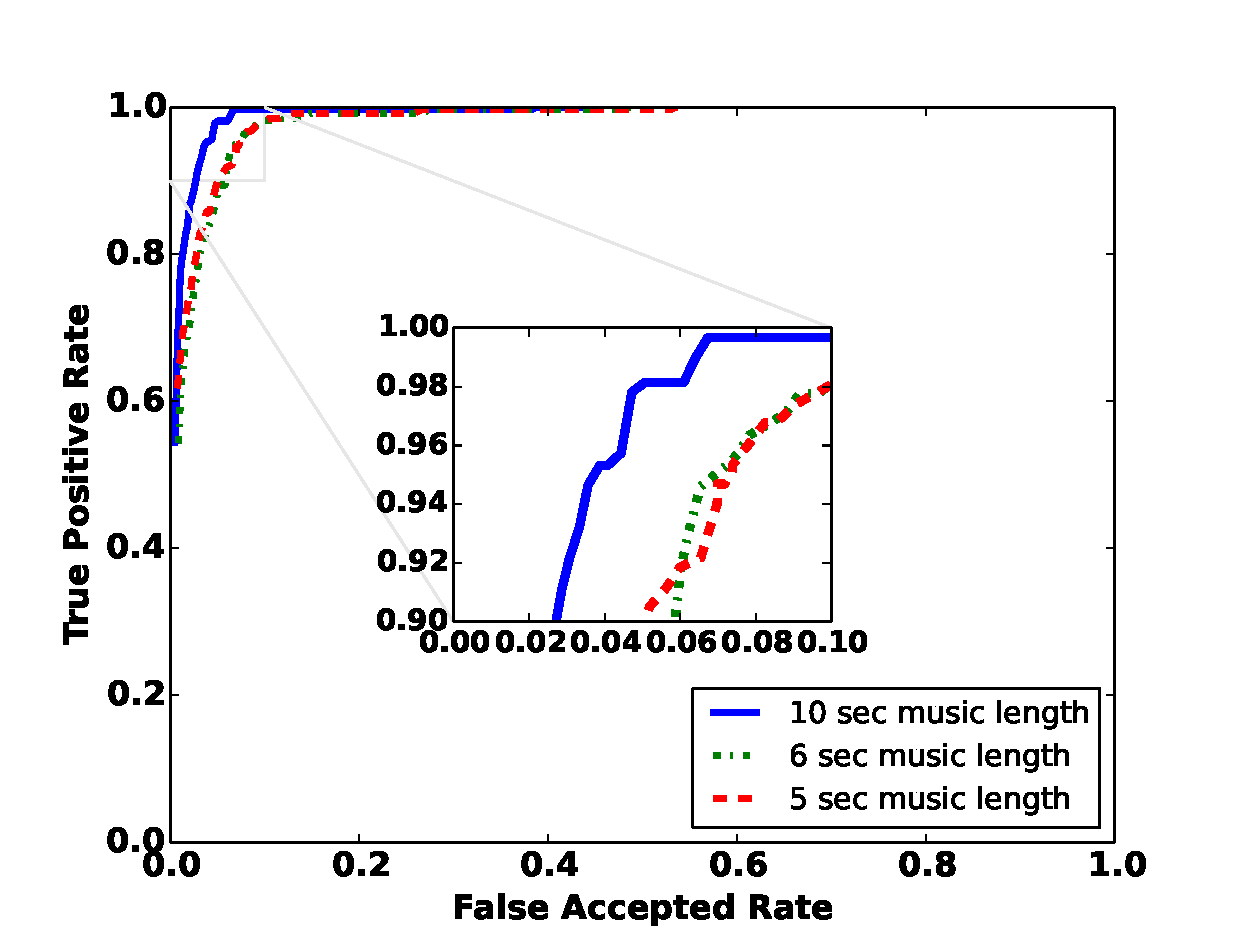
\includegraphics[width=0.3\textwidth]{figure/top1_roc.eps}}
\hspace{0.1mm}
\subfigure[Top 3]{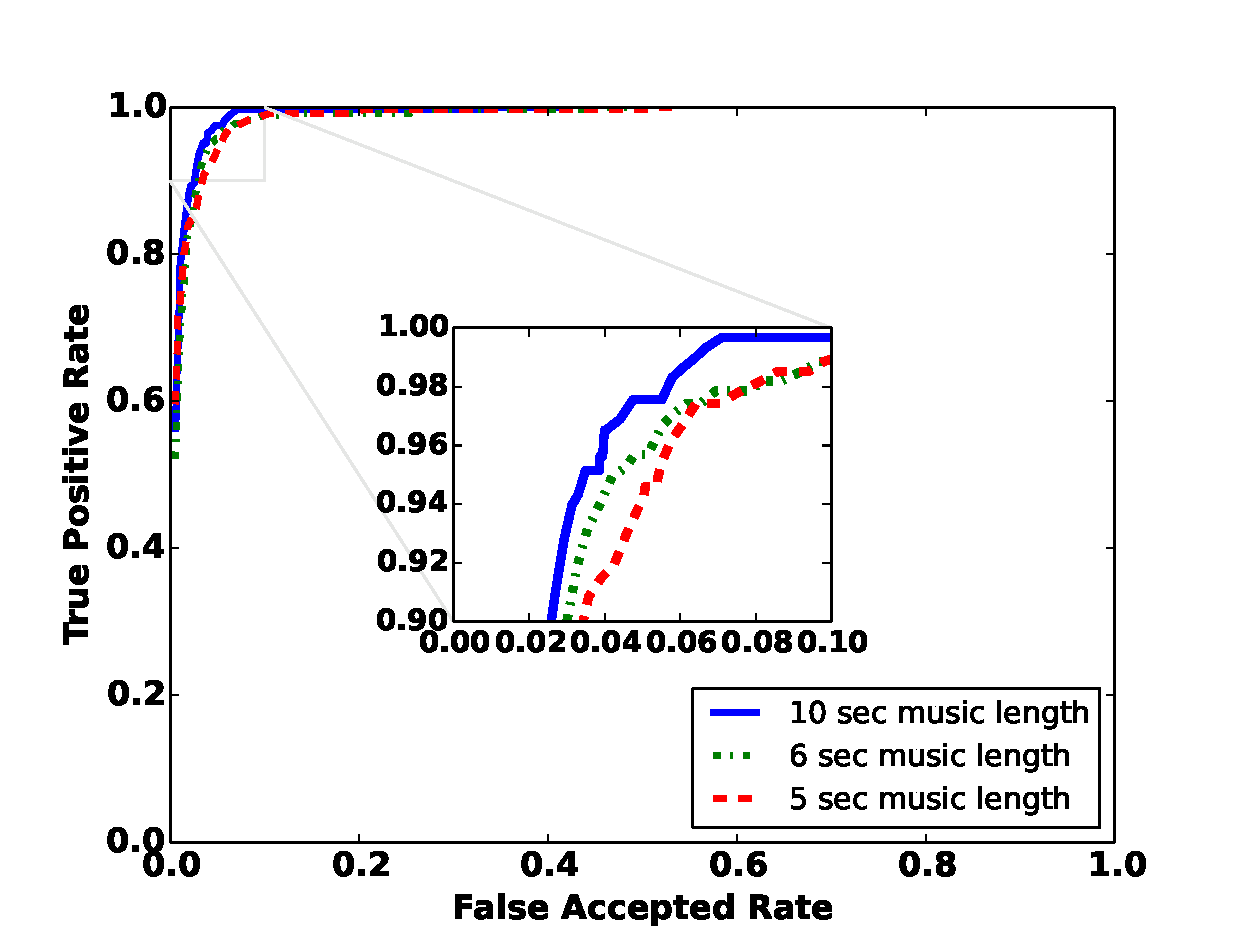
\includegraphics[width=0.3\textwidth]{figure/top3_roc.eps}
 
}
\hspace{0.1mm}
\subfigure[n = 
2.7]{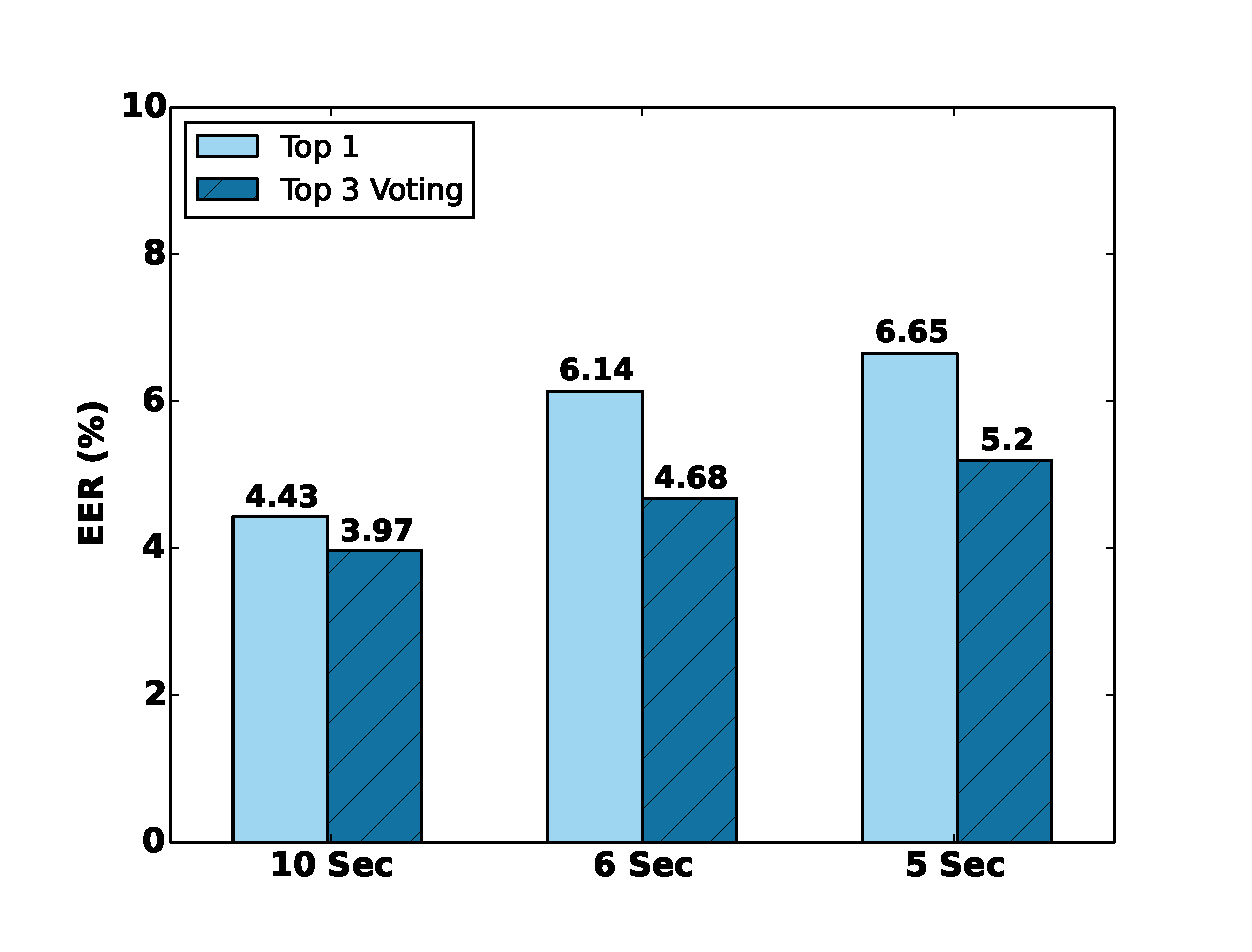
\includegraphics[width=0.3\textwidth]{figure/exp2_vary_length.eps}}
} %end of mbox
\caption{ (a) ROC curves for $K=1$ case, (b) ROC curves for $K=3$ case, (c) 
Equal Error Rate (EER) for Top-1 and Top-3 cases for different music cue 
durations.
In all these plots, the music cue is retained the same (a 10 sec music 
snapshot is trimmed into 10sec, 6 sec and 5 sec accordingly).
}
\label{fig:roc-curves_k}
\end{figure*}
\fi

\begin{figure}[t]
\centering
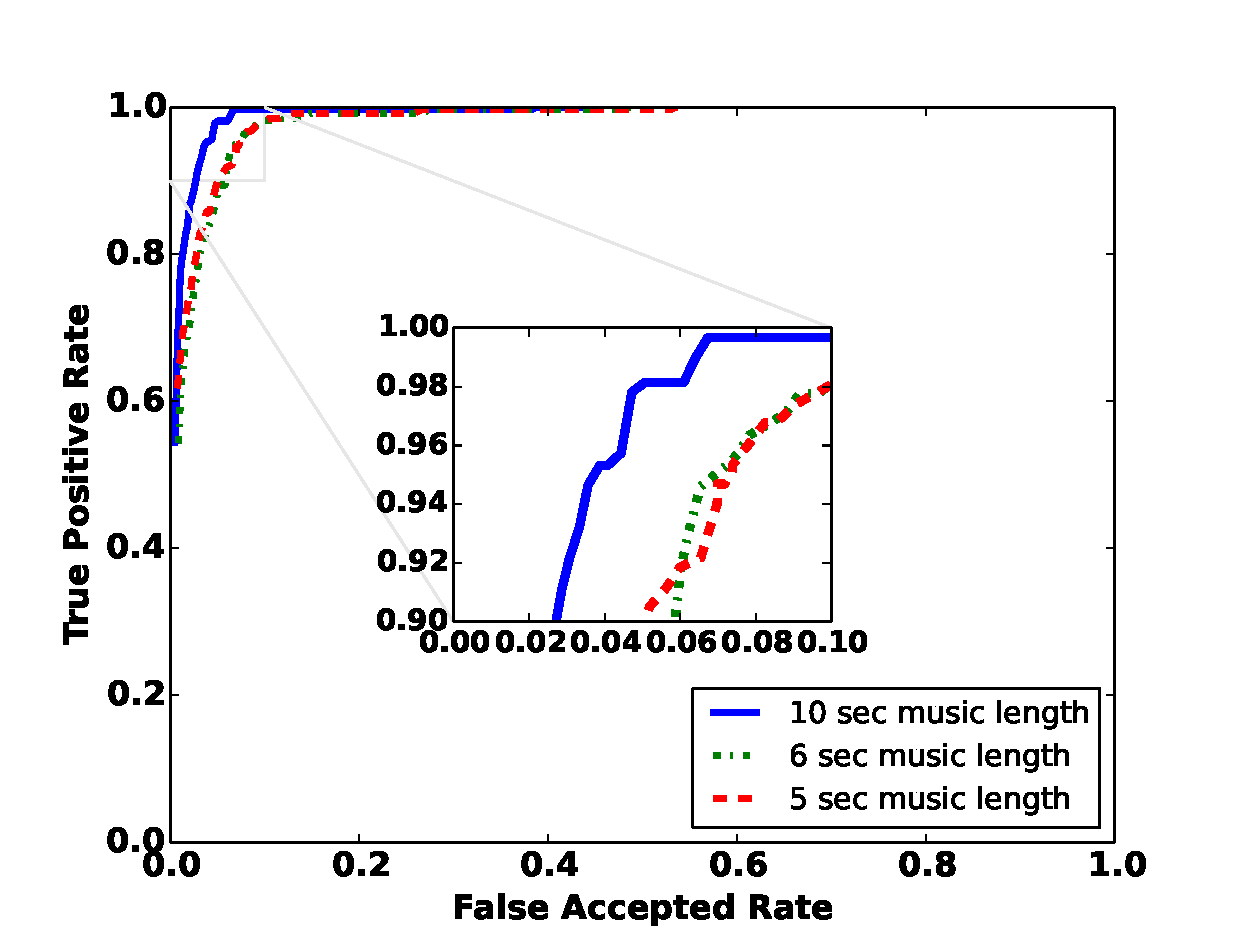
\includegraphics [width=\columnwidth]{figure/top1_roc.eps}
\caption{Evaluation of impact of music cue duration on TPR and FAR in Top-1 
scheme ($K = 1$). A 10 sec music snapshot is trimmed into music cues of 10 
sec, 6 sec and 5 sec correspondingly.The variable here is $n$. Each (TPR, FAR) data point in the curve corresponds to a different value of $n$}
\label{fig:roc-top1}
\end{figure}

\begin{figure}[t]
\centering
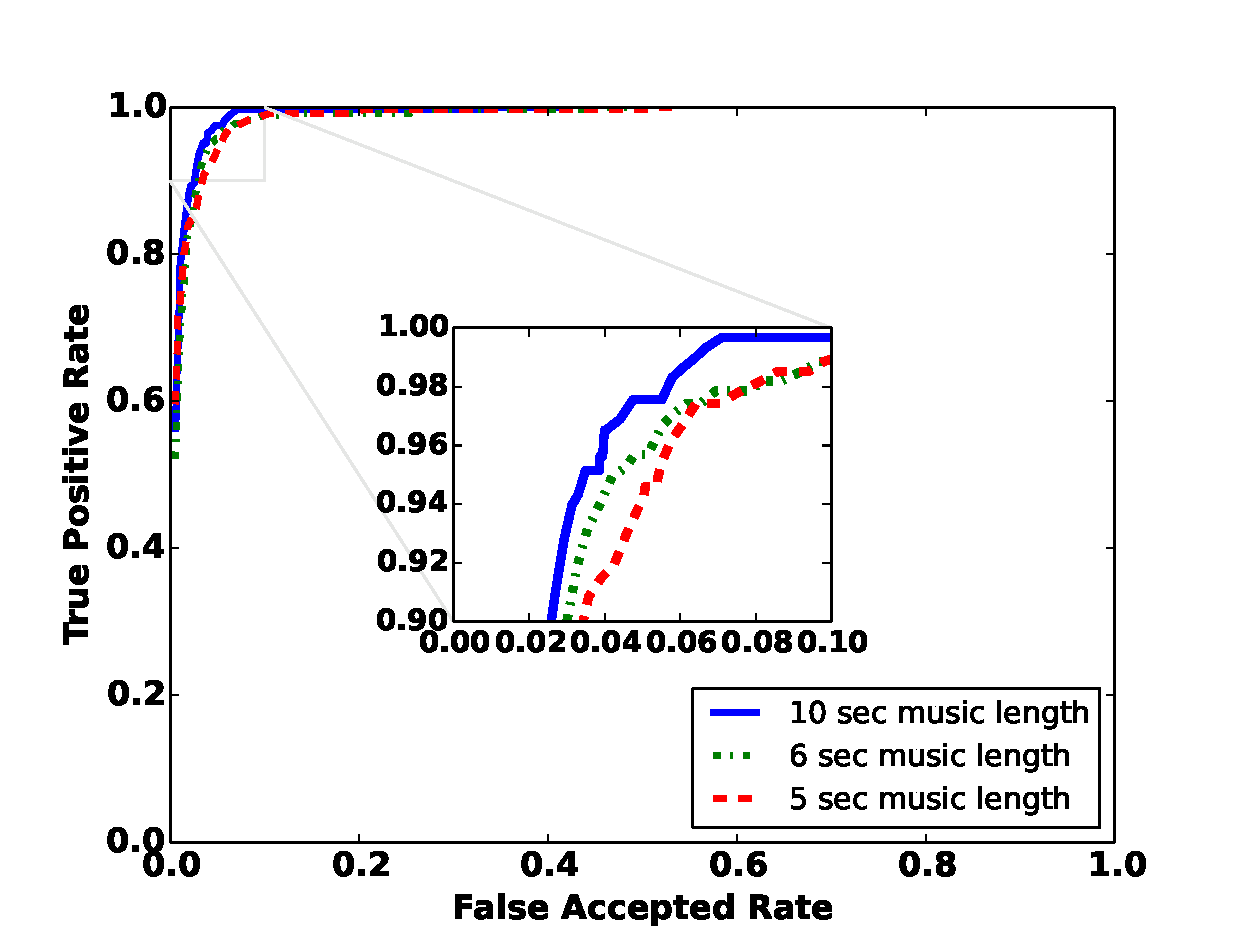
\includegraphics [width=\columnwidth]{figure/top3_roc.eps}
\caption{Evaluation of impact of music cue duration on TPR and FAR in Top-3 
voting scheme ($K = 3$). A 10 sec music snapshot is trimmed into music cues of 
10 sec, 6 sec and 5 sec correspondingly.The variable here is $n$. Each (TPR, FAR) data point in the curve corresponds to a different value of $n$}
\label{fig:roc-top3}
\end{figure}

\begin{figure}[t]
\centering
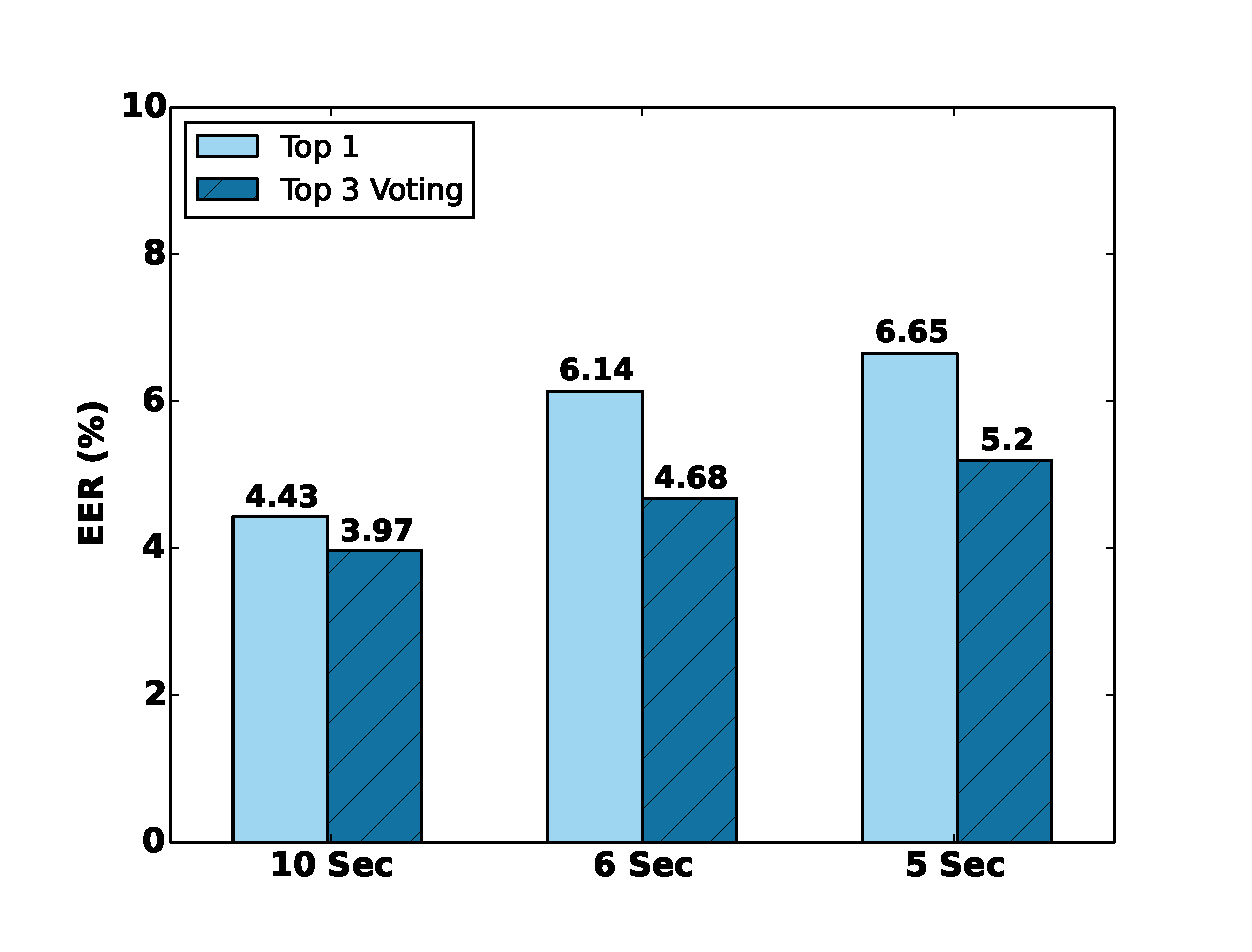
\includegraphics [width=\columnwidth]{figure/exp2_vary_length.eps}
\caption{Comparison of EER for different music lengths (10 sec, 6 sec and 5 
sec) with a fixed n value of 2.7}
\label{fig:eer-length}
\end{figure}

\begin{figure}
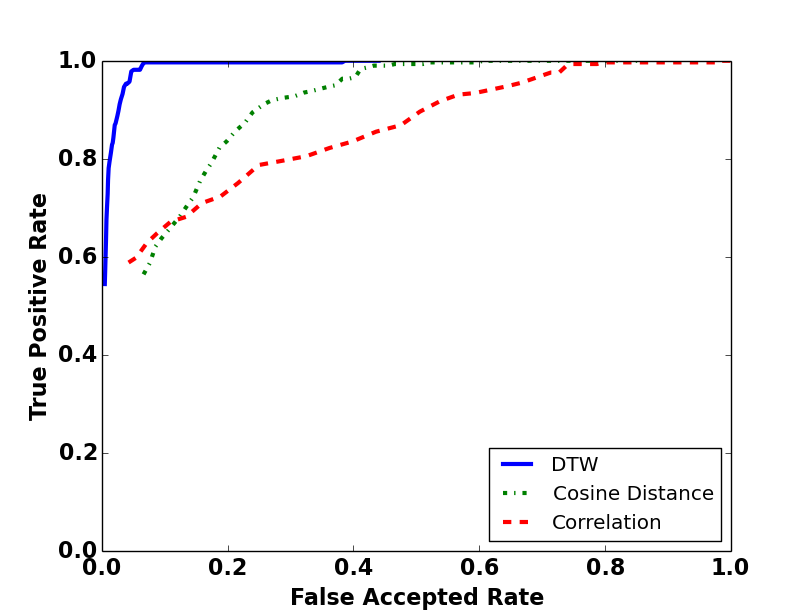
\includegraphics[width=\columnwidth]{figure/roc_dtw_cos_cor.png}
\caption{\label{fig:roc_dtw_cos_cor} Evaluation of impact of different distance metric (DTW, cosine distance, and Correlation). Although DTW is relatively computing-intensive, ROC curve indicates  that DTW provides a large enhancement over the other two metrics. }
\end{figure}

\begin{figure}
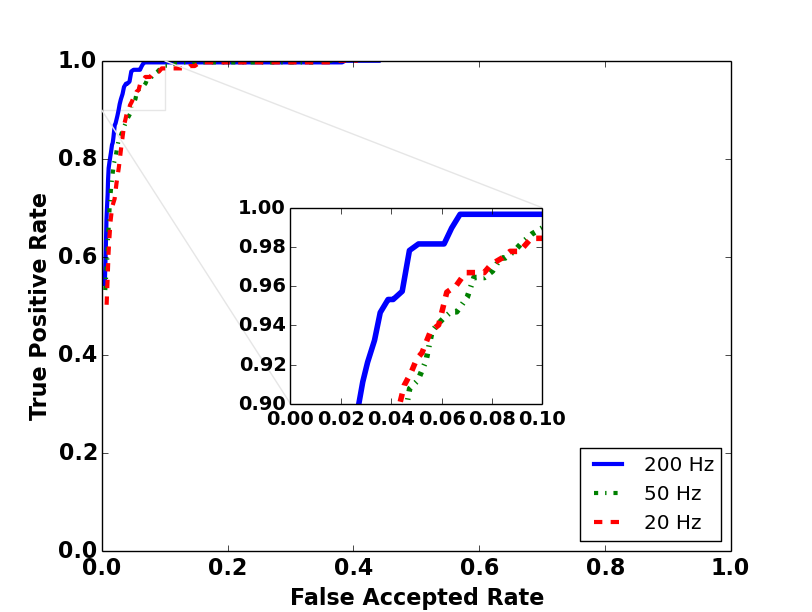
\includegraphics[width=\columnwidth]{figure/roc_dtw_diff_freq.png}
\caption{\label{fig:roc_dtw_diff_freq} Evaluation of impact of different sampling rate shows that the highest sampling rate 200 Hz gives the best resutlt. However, the sampling rate determines computational effort for the smart device, which could be significant in terms of response time.}
\end{figure}


\subsection{Accuracy}
We evaluate the accuracy of \systemname~using metrics that are commonly used 
in evaluating authentication systems, namely,
the false acceptance rate FAR (percentage of false test samples that are 
mistakenly accepted), false rejection rate FRR (percentage of true test 
samples that are mistakenly rejected), and true positive rate 
TPR (percentage of true test samples that are correctly accepted). 
A strict threshold in the classifier can lead to high FRR, while 
overly relaxing the same can lead to a high FAR. Hence, we also consider 
the equal error rate EER (percentage of errors when $FAR = FRR$), that 
considers both FAR and FRR.
%and balanced accuracy BAC, where BAC = 1 - (FAR+FRR)/2.
%We present the accuracy results through the receiver operating 
%characteristics (ROC) curves, TPR versus FAR, as shown in Figures~\ref{} 
%and~\ref{}. 
Figures~\ref{fig:roc-top1}, \ref{fig:roc-top3} and \ref{fig:eer-length} report 
the accuracy 
of \systemname~through the metrics stated above. 
%Figures~\ref{fig:roc-curves} (a)-(c) report the accuracy of 
%\systemname~through the metrics stated above.
In general, our evaluation of the 30 subject data-set indicates that a 
TPR of 95.1\% at FAR of 3.5\%, and EER = 3.97\% can be achieved in 
\systemname, however, these results are tailored to the following parameter 
and algorithm choices:
10 sec music duration, $K = 3$, and 30 (out of 40) trials from each user being 
used for training with a thresholding parameter value $n = 2.7$ with DTW. 
We will now discuss the results and the impact of such parameter choices 
on accuracy in more detail.
\paragraph{Impact of similarity algorithm}
In previous preliminary study, we find that DTW, Cosine Distance, and Correlation are giving promising results for the response time sequence, hence we will evaluate these three algorithms in our end-to-end system. Also due to DTW is relatively more computing-intensive than the other two algorithm, we would like to see whether DTW  is worth of computing resource. In this experiment, we vary thresholding parameter value $n$ and fix the other parameters: 10 sec duration, $K = 1$, and  training data $size = 30$. We can observe from the ROC 
(receiver operating characteristic) curves in Figure~\ref{fig:roc_dtw_cos_cor} that DTW gives the best result among three algorithms, since its curve is the closest to the upper left corner. Our preserves all characteristics of the data, which includes the response time to the music beat and the waveform of 3 axis. In term of matching the waveform of two signal, DTW can achieve significant enhancement than the other two algorithms. 
\paragraph{Impact of music cue duration and $K$ value}

The classification algorithm in \systemname~generates the classification result (YES or NO) by voting among the individual results each generated by the top-K samples in the truing set. We can observe from the ROC curves in Figure~\ref{fig:roc-top1} and \ref{fig:roc-top3} that 
for both, $K=1$ and $K=3$, the TPR is close to 95\% while the FAR is slightly 
above 3\% for the 10 sec music duration. For $K = 1$ the FAR increases to 
about 7\% for the 5 sec and 6 sec cases, however, for $K = 3$ the FAR 
decreases to about 3\% and 4\%, respectively. 
We observe a similar trend with the EER as shown in 
Figure\ref{fig:eer-length}, where improvements of 0.5 - 1 \% 
can be achieved by choosing $K = 3$ over $K = 1$.
This indicates that the accuracy in \systemname~can improve with a larger 
value of $K$. However, the improvement in accuracy through redundancy in the 
training set trades off with the increased execution time as the 
matching requires at least $K - 1$  extra DTW computations as opposed to only 
1 for a top-1 scheme. As we will show ahead, DTW computations incur heavy CPU 
budget on the wearable device. 
%We measure the DTW computation on Google Glass to be the most 
%computationally expensive operation of all the software modules in 
%\systemname.
%\paragraph{Impact of music cue duration}

In general, we observe from the results that the FAR can 
be decreased by increasing the music cue duration. 
We can observe (from Figures~\ref{fig:roc-top1}, \ref{fig:roc-top3} and 
\ref{fig:eer-length}) that the improvement is less significant when the music 
cue duration is increased from 5 sec to 6 sec, however, the improvement is 
more 
significant when the music cue duration is increased to 10 sec. 
In \systemname~the data collection phase for the authentication system 
(sampling accelerometer sensor readings) is executed in parallel with the 
music cue. The data processing phase involving the filtering, classification 
and matching is executed only at the end of the music cue and in the same 
order.
%Hence, execution time of the app will be independent of this duration.
We note that, the data input duration of 5-10 sec for authentication 
may seem long, but in reality, such data input durations are on par with those 
of password based systems~\cite{von2013patterns}.
%We also note that, since the authentication process is initiated only at the 
%end of the music cue, execution time of the app will be independent
%of this duration.

\begin{figure}[t]
\centering
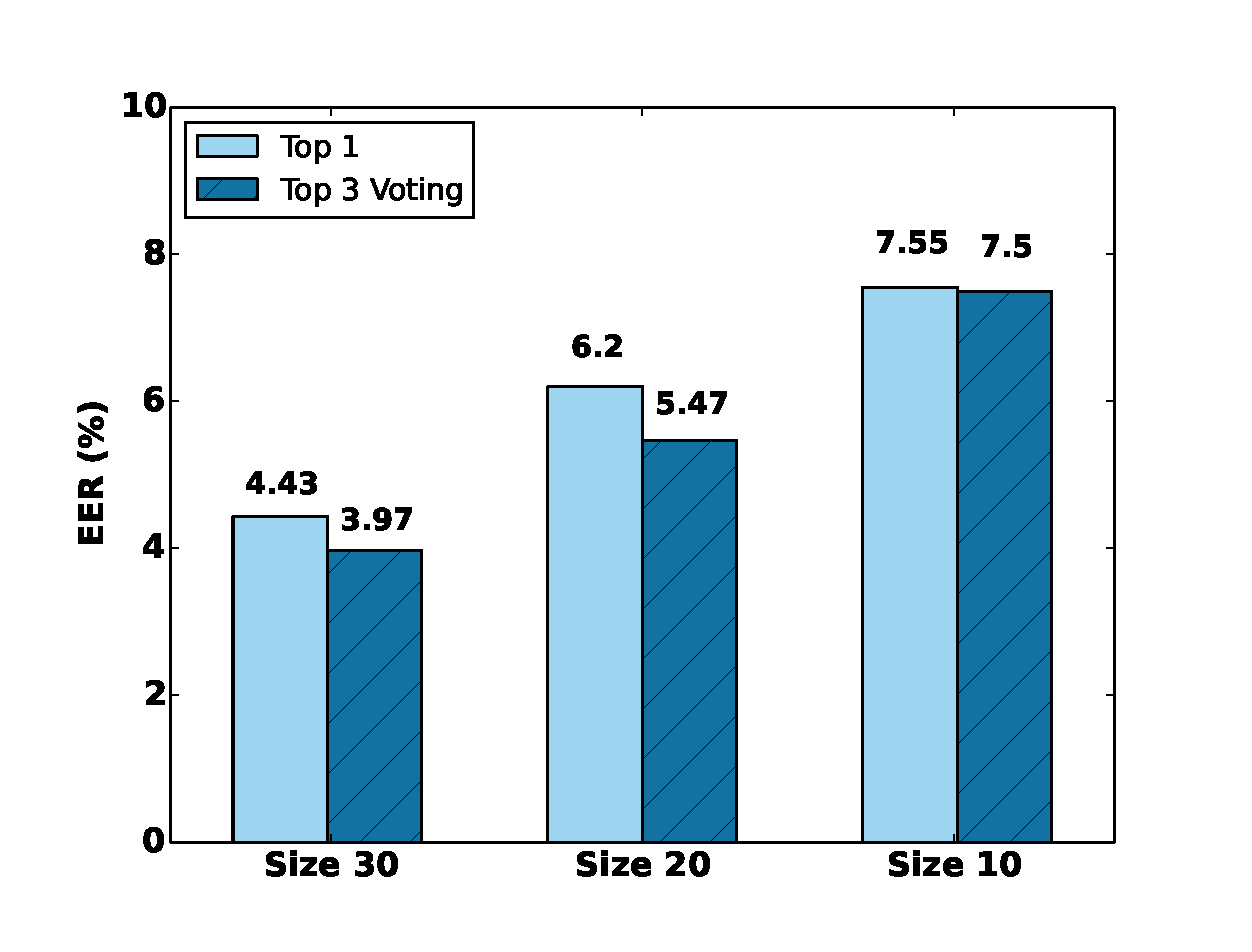
\includegraphics [width=\columnwidth]{figure/exp2_vary_size.eps}
\caption{Comparison of EER for different training sample sizes (30, 20 and 10) 
with fixed n value of 2.7}
\label{fig:eer-size}
\end{figure}


\paragraph{Impact of Training set size}
%The accuracy of detecting and matching the head-movements to the user depend 
%upon the music cue duration, value of $K$, and number of samples used for 
%training.
Recalling from \systemname section~\ref{sec:design}, the input to the training phase
is a set of temporal signals (samples with duration equal to the music cue 
duration), each corresponding to one trial of the head-movements from the 
user. Our evaluations so far considered a training set size of 30 samples. 
In Figure~\ref{fig:eer-size}, we report the EER in \systemname~for three 
different training data set sizes; 10,20 and 30 samples.
We can observe from Figure~\ref{fig:eer-size} that the EER holds an inverse 
relationship with the training set size. A larger training set minimizes the 
variance in mean and standard deviation computations, as the errors in their 
inconsistency are reduced by averaging the mean and standard deviation 
estimates over a larger set of data. 
On the other hand, a larger training set also implies a longer execution time 
of the training phase.
However, in our system design, we posit that the training phase can be 
conducted 
offline on a more compute efficient device (smartphone, PC or server) and that 
the wearable device can pre-fetch the trained data (for example, an XML file), 
prior-to or during data collection phase, through a wireless link.

\subsection{Is it Secured?}
We evaluated the vulnerability by conducting a imitation attack experiment. The reason that these three subjects chosen to become imitated subjects is as following: $Subject A$ performed a simple nodding movement by naturally following the music flow. $Subject B$ also performed a simple nodding, but his response to the music beat always delayed for a certain time, hence other people are not easy to follow. $Subject C$ performed a movement combined with nodding and shaking, and he only nodded/shake at certain beats instead of every beat, which makes his movement is relatively difficult to learn. As shown in Table~\ref{tab:imitation}, 

\begin{table}[]
\centering
\begin{tabular}{lcllc}
\hline
 & \multicolumn{1}{l}{Total Imitator} & \multicolumn{1}{c}{\begin{tabular}[c]{@{}c@{}}Ave. \# of Imitator \\ that Succeed\end{tabular}} & \multicolumn{1}{c}{\begin{tabular}[c]{@{}c@{}}Ave. \# of Trial Before \\ First Successful Login\end{tabular}} & \multicolumn{1}{l}{FAR (\%)} \\ \hline\hline
Subject A & 10 &  &  & 17.67 \\ \hline
Subject B & 13 &  &  & 9.82 \\ \hline
Subject C & 8 &  &  & 3.27 \\ \hline
\multicolumn{1}{c}{Overall} & 31 &  &  & 7.54 \\ \hline
\end{tabular}
\caption{My caption}
\label{my-label}
\end{table}

\subsection{Headbanger Google Glass App Implementation}

\begin{figure}[t]
\centering
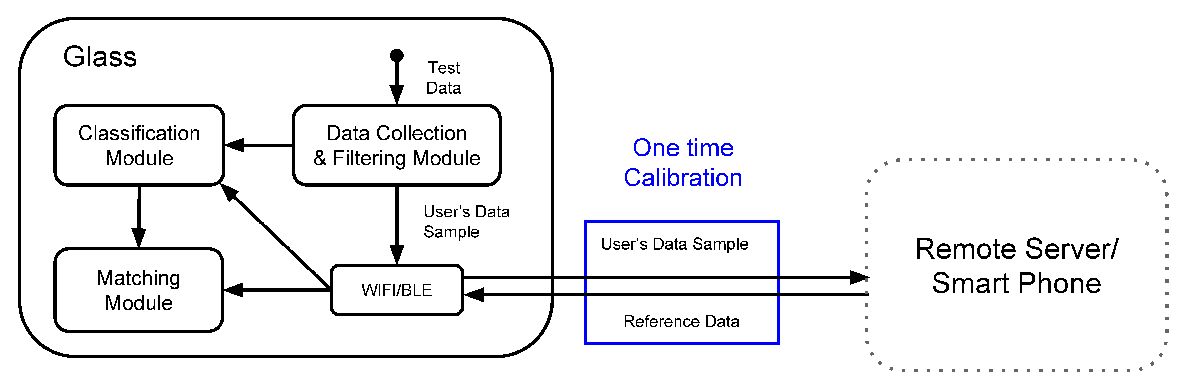
\includegraphics [width=\columnwidth]{figure/software_arch.eps}
\caption{Software modules of \systemname~implementation}
\vspace{25 pt}
\label{fig:glass-softwarearch}
\end{figure}

We implemented \systemname~on Google glass, positioning it as an 
authentication application (app). 
Figure~\ref{fig:glass-softwarearch} shows the main software modules in the 
app. Upon initiation by the user, the app plays a music cue for a stipulated 
duration. The user conducts head-movements in synchrony with the music cue 
while the app records the accelerometer sensor in parallel. At the end of the 
music cue duration the app executes the data processing phase where the 
sensor readings are input to the \systemname's software modules for 
processing. The processing stage includes the filtering of the accelerometer 
sensor values, classification and feature extraction using DTW, and threshold 
based matching of the generated features with those from training set.
%\systemname extracts the head-movement features through 
%the thresholding process discussed in section~\ref{sec:design}, and compare 
%with the feature templates generated from the training phase. 
Upon completion of data processing, the app responds with a YES or NO textual 
output on the Google Glass screen, depending on match score.

In our current implementation, the training phase is conducted offline, prior 
to live-testing off the application.
The training phase involves collecting 30 samples (variable) of the 
head-movement accelerometer readings, generating the features, and saving them 
into a local server (running on PC) as an XML file, with appropriate indexing. 
Upon app initiation on Glass, the trained features are pre-fetched from 
the server through a wireless connection. This ensures that the training set 
is readily available during the authentication process, thus eliminating the 
additional processing time required for the training phase.
Conducting online training, particularly that involves DTW computations, is 
very compute intensive on a resource constrained devices such as Glass. 
One possible solution would be for the Glass to offload the 
training phase computation to a local server machine.
%We reserve such considerations for future implementations.

%Among all the software modules, the ``training set construction model'' is 
%the most computing-intensive, and as a result, we executed the model on the 
%bluetooth-paired smartphone. The rest of the modules are implemented and 
%executed on the glass. 
%In our on-glass app, the classification module runs the 
%thresholding-based classification. 
\subsubsection{Response time}

\begin{table}
\begin{tabular}{|ccclc|}
\hline
\multicolumn{1}{|c|}{\multirow{2}{*}{\begin{tabular}[c]{@{}c@{}}music  cue \\ 
duration (s)\end{tabular}}} & 
\multicolumn{1}{c|}{\multirow{2}{*}{\begin{tabular}[c]{@{}c@{}} response\\ 
time (s)\end{tabular}}} & \multicolumn{3}{c|}{time breakdown (\%)}             
\\ \cline{3-5} 
\multicolumn{1}{|c|}{}                                                         
                             & 
\multicolumn{1}{c|}{}                                                          
                              &
 Filtering & \multicolumn{1}{c}{DTW} & Thresholding   \\ 
 \hline\hline
10                                                                             
                             & 
4.4                                                                           
                              &
 0.20      & 99.80                   & \textless0.01  \\
6                                                                              
                             & 
2.73                                                                           
                              &
 0.26      & 99.74                   & \textless0.01  \\
5                                                                              
                             & 
2.44                                                                           
                              &
 0.28      & 99.72                   & \textless 0.01 \\ \hline
\end{tabular}
\caption{\label{tab:glass} Measured response time of \systemname~app implementation on Google 
Glass with different music cue durations and for $K = 1$. The response time 
reported here is an average over 20 trials.}

\end{table}

In Table~\ref{tab:glass} we report the measured average response-time 
of the \systemname implementation on Google Glass app for music cue durations 
of 5,6 and 10 seconds. We conducted the benchmark execution-time profiling of 
\systemname~on Glass in a controlled indoor laboratory setting with no 
mobility. We define response time as the time elapsed between music cue 
completion to 
the display of authentication response (YES/NO text) on the Glass screen. 
Our measurements indicate that the response time is within 5 seconds for a 10 
second data input, and is almost halved for a 5 second data input.
We feel that a response time of 2-5 sec for a local authentication solution in 
Google Glass is comparable to that of prior-art that comes close to our 
solution~\cite{von2013patterns,egelman2014you}.
It is also important to note that authentication solutions that execute 
locally on head-worn wearable devices, especially on a heavily resource 
constrained device like Glass, are still not mature. However, the hope is that 
such solutions will possibly catch up to speed in the near future and that our 
approach is advancing one step in that direction. 
In Table~\ref{tab:glass} we also report the execution time of the key 
processes in \systemname; filtering, DTW computation ($K = 1$ requires 1 DTW 
computation), thresholding based similarity matching. 
We can observe from Table~\ref{tab:glass} that the DTW computation 
dramatically compute intensive than the other processes. 

It is important to note that our current implementation uses a faster 
version of the DTW algorithm called Fast DTW~\cite{salvador2007toward}, 
providing about 2x speed-up in DTW computation.
We believe that the response time can be reduced 
further through strategic methods such as, further optimizations in the Fast 
DTW algorithm or pipelining the app execution along with data collection.
A specific strategy for reducing response time for rejected attempts can be 
that, after a short duration, before the entire music cue is played, if it is 
found that a user's movement does not match the signature of the claimed user
with a sufficient pre-determined confidence level, then the on-site 
classification may be terminated instead of waiting for the entire duration to 
yield the rejection.
Another example, may include cyber-foraging strategies to offload heavy
computation tasks, such as online training and classification, to the user's 
Bluetooth paired smartphone or a nearby cloudlet~\cite{ha2014towards}.


\section{Discussion}\label{sec:disc}

In this study, we showed that head-movements have the potential to be used as
a reliable behavioral signature for user authentication.
We will now discuss some of the limitations that we identified from this work
and prospects for future work as below.

\iffalse
\subsection{Reliability}
Our work in this paper shows that head-movements are distinctive and
repeatable in controlled settings. However, in reality, the behavior of
head-movement signatures over chaotic settings will be a key factor to decide
on the effectiveness of this approach. Our work only evaluates the case when a
user is in a stationary setting when attempting to login, such as when sitting
on the chair or standing still. The performance of this approach in realistic
mobile settings such as walking or in a vehicle is yet unknown. It is also
unclear if the head-movement patterns are repeatable in such a mobile environment, or
if the ambiguities of vehicle motion versus head-motion can be separated. 
%%For example, we don't know whether a person's
%%head-movement signature will be the same no matter whether she is sitting,
%%standing still, walking, running, or driving.
%%The most important concern is the reliability of human head-movements. Even
%%though we have shown that head-movements are rather distinctive and
%%repeatable
%%in a controlled setting, it is yet unclear how it will perform in realistic,
%%but chaotic settings. For example, we don't know whether a person's
%%head-movement signature will be the same no matter whether she is sitting,
%%standing still, walking, running, or driving.
Similarly, a person's head-movement signature may also depend on the mood/energy level of
the person; for example, a fresh and energetic user may provide significant
head-movements as compared to a sick or tired user whose signatures may not
even be detectable. Inconsistencies in the accelerometer sensor such as drift and temporal bias can
significantly affect the nature of inferred head-movement signature.
Head-movements, on the other hand, may also evolve over time for a person
which call for periodic calibration of the system and/or the training data.
%To address these two temporal changes, we may need to periodically
%recalibrate
%the sensors and dynamically adjust our training data to reflect new movement
%trends.
While reliability metric was out of the main scope of this paper, we are keen
to address the same in future work.
\fi

\subsection{Power consumption}

\begin{table}
\centering
\begin{tabular}{lccc}
\hline
Component    & Power Consumption (mW) & Duration (s)       \\ \hline\hline
Sensor  & 29                    & 10       \\
Speaker & 410                    & 10      \\
CPU      & 1600                   & 14.4 \\ \hline
\end{tabular}
\caption{Power consumption on Google Glass of components relevant to 
\systemname.  The CPU (running at 
maximum frequency) power consumption includes that of the heads-up display 
screen being ON as well. Duration marks the time for which
component was ON during the a 10 sec music cue length trial}
\label{tab:pow}
\end{table}

Google Glass is an example of a wearable device that is heavily battery power 
constrained. Measuring the power consumption of the Glass's battery is a 
challenging task as that requires physically dismantling the device. 
We refer to the measurement paper on Google Glass by Robert et. 
al~\cite{likamwa2014draining} for the power consumption of the 
key components relevant to \systemname~implementation on Glass: the speaker 
for music cue playback, the accelerometer sensor and the CPU being ON during 
the entire authentication process. We report the relevant numbers in 
Table~\ref{tab:pow}. While the high CPU power consumption may not necessarily 
be surprising, the speakers also extrude considerable energy from the battery. 
We note that one possible solution for future consideration would be to play 
the music cue as intermittent notes over the duration, for example a ping or a 
beat sound periodically, where the speaker would be switched ON only during 
playback.

\subsection{Is this secure?}
An authentication system must have an effective protocol ensuring security of 
the authenticating user's data. Our system runs an implicit
authentication protocol where the user is given a finite set of (calibrated) 
music tracks to pick, based on which the user makes head-movements that are 
used as unique signatures for authentication.
Our design assumes implicit security of the user's data, as a
user voluntarily accepts the enforcement of conducting head-movements  
in response to the music. It is arguable that such enforcements are an 
integral part of most commonly used authentication systems; for example, 
typing a password, swiping the finger on the fingerprint sensor, approving of 
the camera recognizing the face. In all these cases the user is aware 
that he/she is inputing data into the system for authentication.

One way of compromising security would be a successful spoof of the 
head-movement by an adversary. For example, head-movements from an authorized 
user may be imitated by an adversary attempting to login to the device. 
%However, this requires that the wearable device is physically accessible to 
%the adversary. Since head-worn devices are at the visual field of view of the 
%user the chances of it getting lost or being stolen will be lower than other 
%wearable devices such as smart-watch or smart-necklaces. 
If the head-movements from the user is regular (such as a nod), it may be 
easily imitated as opposed to a random head-shake such as a head-bang.
To understand the effect of imitation on the accuracy of authenticating a user 
to \systemname, we conducted an experiment (under the same set up as  
described in section~\ref{sec:results}) where 29 volunteer participants 
were asked to imitate the head-nod movements of one user (one of the authors) 
who was trying to authenticate to the device using a 10 sec music cue. A total 
of 30 trials were conducted of which 10 samples were used as test data and 20 
for training. Our evaluations of this dataset resulted in reasonable accuracy 
values of, an 
EER of 7.2\% and a balanced 
accuracy $BAC = 1 - ((FAR+FRR)/2)$ of 94.5\% for the authorized user. Our 
results indicate that attacking the system through imitation of a simple 
head-gesture can still be challenging.

%A seamless design
%would ensure that the system captures even the slightest of the subconscious
%head-movements in the event that the user does not make any enforced
%head-movements. In such cases the head-movement signatures will have to be
%much more elaborate with multiple attributes that correspond to the different
%realistic use-cases of the system.

\subsection{Multi-Modality}
Inconsistencies in the accelerometer sensor such as drift and temporal bias can
significantly affect the nature of inferred head-movement signature.
Head-movements, on the other hand, may also evolve over time for a person
which call for periodic calibration of the system and/or the training data.
The array of motion sensors (accelerometer, gyroscope, inertial measurement 
unit) open up opportunities for multi-modal motion sensing. For example,
in Glass, accelerometer data can be combined with gyroscope measurements to 
provide multi-dimensional head-movement features that can improve the quality 
of the inferred signatures. Head movements can also be combined with other 
body movements to generate valuable, reliable signatures for authentication. 
%Additionally, head-movement is just one type of body movements, and we can
%investigate other types of body movements as well.
For example, through a simple test experiment using the Google Glass
infra-red (IR) light sensor (we had to root the Google Glass to access the
IR sensor unit) we observed that the blinking and winking patterns of users in
response to the music stimulus were reasonably differentiable among users.
Such patterns may also independently serve as another biometric that can be
used for authentication purpose, or can be combined with head-movements for better results.
Recent studies have shown that heart beat or pulse can also serve as reliable
biometric for authentication purposes~\cite{hernandezbioglass,nymi}.
We reserve such potential enhancements to our system for future implementation.
%A recent study has shown that Google glass can detect human heart
%beat~\cite{hernandezbioglass}; heartbeats can thus be
%used as another biometric.
%If extra hardware can be introduced, then more movement patterns,
%such as eye movement, can be leveraged as well.

\iffalse
\subsection{Seamless Protocol}
An authentication system must have an effective protocol for authenticating
users seamlessly to their device. Our system runs a simple authentication
protocol where the user is given a finite set of (calibrated) music
tracks to pick, and based on which the user makes head-movements in response.
Our design assumes that the user voluntarily accepts the enforcement of the
requirement of head-movements in response to the music. A seamless design
would ensure that the system captures even the slightest of the subconscious
head-movements in the event that the user does not make any enforced
head-movements. In such cases the head-movement signatures will have to be
much more elaborate with multiple attributes that correspond to the different
realistic use-cases of the system.
%Our protocol can consist of several steps. In the first step, the user will
%be
%asked to choose a user name from all the legitimate users of the device.
%Then,
%the user will be asked to select the favorite music track of the claimed
%user.
%If the selection is correct, the device will play the music and ask the user
%to move along (including head movement, eye blinking/winking, etc). ***YZ:
%what else??? ***
\fi

\iffalse
\subsection{Processing/Battery Power Constraints}
Battery power consumption and computing power are very important parameters
for consideration when optimizing a design to accommodate to wearable devices.
Wearables usually have serious resource limitations, especially in terms of
processing power and battery power.
This paper, addresses these concerns through optimization strategies in the
head-movement signature classification stage of the proposed authentication
algorithm. For wearables it is important that such optimization strategies are
taken to next levels until a roadblock is reached.
%In this paper, we have considered a set of
%optimization techniques to reduce the processing demand as well as power
%consumption, e.g., testing against top $K$ samples instead of  the entire
%training set, using thresholding-based classifier instead of SVM classifier.
For example, one such strategy extension in this work can be that, after a
short duration, before the entire music is played, if it is found that a
user's movement does not match the signature of the claimed user
with sufficient confidence level, then the on-site classification may be
terminated  instead of waiting for the entire duration to yield the rejection.
Another example, may include cyber-foraging strategies to offload heavy
computation tasks, such as classification, to the user's Bluetooth paired
smartphone.
\fi

\subsection{Large Scale User Study}
To be adopted as a primary authentication mechanism on smart-glass devices,
the technique will have to be evaluated over a large number of usage and
and over a large user base. Conducting such rigorous large-scale experiments
is typically infeasible in academic laboratory settings. We reserve such
large scale experiments for future work, and hope to accomplish through
industry collaborations. We will, however, be releasing our data-sets to the 
public in the near future.
\section{Related Work}\label{sec:related}
Headbanger is a behavioral biometric based
authentication system, which focuses on head movement. 
%To our best knowledge, it is the first wearable authentication system that 
%only relies on accelerometer signatures from human \emph{head} motion. 
Below, we review the related literature on mobile device authentication.

%in wearable/mobile device based schemes, infrastructure based
%schemes, and biometric-rich based schemes.

%\subsection{Wearable/mobile device based schemes}
The work by Harwin et al.~\cite{harwin1990analysis} is usually considered the 
first to propose use of head gestures by combining pointing and movements
for human computer interaction. 
In~\cite{westeyn2004recognizing}, the authors used 
eye-blinking pattern as a unique feature for
authentication. They achieved 82.02\% accuracy with 9 participants. Compared 
to eye blinking pattern, head-movements can provide much more entropy, 
therefore can be considered as a more suitable biometric characteristic. 
The work by Ishimaru et al.~\cite{ishimaru2014blink} comes close to our system 
design; they proposed to combine the eye blinking frequency from the infrared 
proximity sensor and head motion patterns from accelerometer sensor on Google 
Glass to recognize activities (e.g., reading, talking, watching TV,
math problem solving) 
The key difference of our approach from ~\cite{ishimaru2014blink} is 
that, their approach focused on common head-movement and eye-blink patterns 
when people employ the same activities such as reading, typing, etc. 
We carefully investigated the head-movements from human subjects and found 
that they are unique to each person. 
Our system also identified these head-movements with a higher accuracy (95$\%$ 
versus 82$\%$ in ~\cite{ishimaru2014blink}).

There are also a number of physiological activity recognition studies 
using computer vision~\cite{kjeldsen2001head,hernandezbioglass}. 
While~\cite{kjeldsen2001head} primarily uses computer vision to detect 
head gestures, BioGlass~\cite{hernandezbioglass}
combines Google Glass's accelerometers, gyroscope, and camera to
extract physiological signals of the wearer such as pulse
and respiratory rates. Camera processing on wearable devices, especially 
Google Glass is compute intensive and has a high energy 
budget~\cite{likamwa2014draining}.

Accelerometers have long been used to sense, detect and also recognize
movements in other parts of the body; for example, gait recognition requires 
sensing in areas such as waist~\cite{ailisto2005identifying},  
pocket~\cite{gafurov2007gait}, arm~\cite{okumura2006study,gafurov2008arm},
leg~\cite{gafurov2006biometric} and ankle~\cite{gafurov2011user}.
These techniques, though well known, may not be suitable for on wearable 
devices due to complexity (computation and energy) in the machine learning 
process.
%They are similar in that they collect the raw accelerometers data
%and apply signal processing and/or machine learning techniques  to perform
%authentication.

Hand gesture and touchscreen dynamics are often coupled for
authenticating to a (touchscreen) device. A number of contextual features
including biometrics~\cite{sae2012biometric} (e.g. finger length, hand size,
swipe/zoom speed, acceleration, click gap, contact size, pressure)
and behavioral feature (e.g. touch location, 
swipe/zoom length,
swipe/zoom curvature, time, duration) have been exploited as
effective features for authentication 
purpose~\cite{frank2013touchalytics,cai2013mobile,feng2014tips}.
While most of the techniques require users to explicitly conduct a
gesture following a specific pattern, TIPS~\cite{feng2014tips}
proposed a multi-stage filtering with dynamic template adaptation
strategy to perform the user authentication in uncontrolled
environments -- when a users naturally their phone. 

There is indeed a significant prior art in authentication system 
implementations using various techniques such as 
speech~\cite{reynolds2000speaker}, computer vision and image
~\cite{bowyer2006survey}, graphical passwords~\cite{biddle2012graphical}, 
gestures~\cite{sherman2014user}, biometric 
fingerprints~\cite{jain1997identity}. 
In this paper, we do acknowledge the viewpoint that our approach can also be 
used as a complementary scheme to most of the existing techniques in the 
authentication application space.

%It was extended by Kjeldsen~\cite{kjeldsen2001head} to more
%categories such as continuous control, spatial selection and
%symbolic selection

%Gafurov et al.~\cite{gafurov2006biometric} developed a wearable
%biometric gait authentication system. The sensor is attached to the
%lower leg to extract the gait patterns -- accelerations in three
%directions: vertical, forward-backward and sideways motion of the
%lower leg. A combination of these accelerations is used for
%authentication. ~\cite{gafurov2011user} ankle
%\subsection{Infrastructure based schemes}

%\subsection{Biometric-rich based schemes}
%Fingerprints

% are we the first one? the cloest work? how far we are going to reach out? categories in general: image? voice? touch?
% on glass; body movement;

%mobisys 2014 papers

%gesture based authentication

%Music based movements -- GaTech

%Japanese paper on google glass and eye-wink

%hardware fingerprinting -- check CCS 2014

%acc-based authentication
%http://ieeexplore.ieee.org/xpl/articleDetails.jsp?arnumber=5634532&sortType%3Dasc_p_Sequence%26filter%3DAND%28p_IS_Number%3A5634461%29

%wearable security
%http://gaia.cs.uiuc.edu/papers/wss.pdf

%commercial solutions: Nymi -- eyewink blink pattern

%BioNym -- heartbeat

\section{Concluding Remarks and Future Direction}
\label{sec:conc}
As wearable devices are increasingly weaved into our everyday life, providing security to the data acquired by or accessed through these devices becomes critically important. In this study, we have developed a user authentication system that uses head-movement patterns for direct
authentication to a wearable device. Compared to existing authentication solutions, the proposed solution delivers accurate authentication, is robust against imitation attacks, incurs low processing delays, and offers great convenience to users.

%We developed a light-weight approach that
%infers head-movements of users in response to music and generates signatures
%that are unique to every user.
%Our technique specifically uses the dynamic time-warping (DTW) tool to
%generate a head-movement feature that contains the mean and standard
%deviation of the DTW score of each user, determined over a multiple-user data
%set. The matching is conducted based on a thresholding scheme.
%Experimental observations revealed that the head-movement signatures generated
%using the dynamic time-warping tool, in response to the same music track, were
%consistent in typical stationary environments such as user sitting or
%standing at one location while attempting to authenticate. We leveraged the
%consistency in the head-movement signatures to develop two classification
%algorithms, based on machine learning and adaptive thresholding, to
%efficiently and accurately label user signatures.
Through an extensive evaluation that involves 95 users, we observe that the
average true acceptance rate of our approach is at 95.57$\%$ and the false
acceptance rates at 4.43$\%$. We also observe that even simple head-movement patterns only allow less then 3\% of the imitation attacks to succeed. We have also implemented an app on Google Glass, and measured the end-to-end processing delay of less than 2 seconds for a 10-second data sample. As a result, we believe it is realistic for the proposed authentication system to be executed on resource-constrained devices such as smart-glass. We further believe the proposed method can help enable wider deployment of wearable devices and apps in our life. Towards this goal, in our future work, we will focus on how to make the head-movement based user authentication approach more reliable in real-world settings.

%We have also optimized our algorithms to
%minimize the processing latencies and power consumption, making them suitable
%for wearable devices.
%The multi-user data sets were validated and verified during the
%course of our evaluations and will be released for public use in near future.

\iffalse
In this paper, we present the design, implementation and evaluation
of Headbanger, a head gesture based authentication system.
Headbanger generates a signature from user's head-movements in
response to short duration of audio track with fast beats, and uses
this signature as the behavioral biometric for authentication.
Through extensive experiments on the prototype on Google Glass
involving ?? users, we demonstrated that Headbander can achieve **\%
accuracy and thus with proper audio stimuli, head-movement alone
will be reasonably sufficient to serve a effective behavioral
biometric for authentication. We believe this work will be the basis
for using audio catalyst to enrich more useful human contextual
applications.
\fi 

\balance
%\scriptsize
%\footnotesize
%\small
%\bibliographystyle{acm-sigchi}
\bibliographystyle{abbrv}
\bibliography{sugang}
\end{document}